%! TEX root = **/000-main.tex
% vim: spell spelllang=en:

%%%%%%%%%%%%%%%%%%%%%%%%%%%%%%%%%%%%%%%%%%%%%%%%%%%%%%%%%%%%%%%%%%%%%%%%%%%%%%%%
% PREAMBLE
%%%%%%%%%%%%%%%%%%%%%%%%%%%%%%%%%%%%%%%%%%%%%%%%%%%%%%%%%%%%%%%%%%%%%%%%%%%%%%%%
%! TEX root = **/000-main.tex
%%%%%%%%%%%%%%%%%%%%%%%%%%%%%%%%%%%%%%%%%%%%%%%%%%%%%%%%%%%%%%%%%%%%%%%%%%%%%%%%
%% LaTeX preamble, load in main.tex with: \input{preamble}
%%%%%%%%%%%%%%%%%%%%%%%%%%%%%%%%%%%%%%%%%%%%%%%%%%%%%%%%%%%%%%%%%%%%%%%%%%%%%%%%

\documentclass[12pt]{report}
% \documentclass[12pt,draft]{report}

\usepackage[a4paper, left=2.5cm, right=2.5cm, top=2.5cm, bottom=2.5cm]{geometry}

% for debugging overfulls
%\documentclass[draft, 12pt, oneside]{article}
%\usepackage[showframe, a4paper, left=2.5cm, right=2.5cm, top=2.5cm, bottom=2.5cm]{geometry}

%%%%%%%%%%%%%%%%%%%%%%%%%%%%%%%%%%%%%%%%%%%%%%%%%%%%%%%%%%%%%%%%%%%%%%%%%%%%%%%%
%% FONTS
%%%%%%%%%%%%%%%%%%%%%%%%%%%%%%%%%%%%%%%%%%%%%%%%%%%%%%%%%%%%%%%%%%%%%%%%%%%%%%%%

\usepackage[T1]{fontenc}
\usepackage{fontspec}
\usepackage{microtype}

\setmonofont[Scale=MatchLowercase]{DejaVu Sans Mono}

%%%%%%%%%%%%%%%%%%%%%%%%%%%%%%%%%%%%%%%%%%%%%%%%%%%%%%%%%%%%%%%%%%%%%%%%%%%%%%%%
%% MATHS
%%%%%%%%%%%%%%%%%%%%%%%%%%%%%%%%%%%%%%%%%%%%%%%%%%%%%%%%%%%%%%%%%%%%%%%%%%%%%%%%

\usepackage{amsthm}     % Theorem enviroment
\usepackage{amssymb}    % More symbols
\usepackage{amstext}    % Text inside mathenv
\usepackage{mathtools}  % amsmath + more

%\usepackage{relsize}    % Bigger math with mathlarger{___}
%\usepackage{nicefrac}   % nice fractions in one line

%\usepackage{IEEEtrantools} % Complex equation arrays


%%%%%%%%%%%%%%%%%%%%%%%%%%%%%%%%%%%%%%%%%%%%%%%%%%%%%%%%%%%%%%%%%%%%%%%%%%%%%%%%
%% LANGUAGE
%%%%%%%%%%%%%%%%%%%%%%%%%%%%%%%%%%%%%%%%%%%%%%%%%%%%%%%%%%%%%%%%%%%%%%%%%%%%%%%%

\usepackage{polyglossia}
\setdefaultlanguage{english}
\setotherlanguages{spanish,catalan}

%%%%%%%%%%%%%%%%%%%%%%%%%%%%%%%%%%%%%%%%%%%%%%%%%%%%%%%%%%%%%%%%%%%%%%%%%%%%%%%%
%% BIBLIOGRAPHY
%%%%%%%%%%%%%%%%%%%%%%%%%%%%%%%%%%%%%%%%%%%%%%%%%%%%%%%%%%%%%%%%%%%%%%%%%%%%%%%%

\usepackage[
    backend=biber,
    style=numeric,
]{biblatex}
\DeclareNameAlias{default}{family-given}

\addbibresource{biblio.bib}

\usepackage{fvextra}        % Req by minted (must load before csquotes)
\usepackage{csquotes}       % For bibliography quotations
\DeclareQuoteAlias{spanish}{catalan}

%%%%%%%%%%%%%%%%%%%%%%%%%%%%%%%%%%%%%%%%%%%%%%%%%%%%%%%%%%%%%%%%%%%%%%%%%%%%%%%%
%% COMMON
%%%%%%%%%%%%%%%%%%%%%%%%%%%%%%%%%%%%%%%%%%%%%%%%%%%%%%%%%%%%%%%%%%%%%%%%%%%%%%%%

\usepackage[dvipsnames]{xcolor}

\usepackage{graphicx}   % graphics
\graphicspath{{./figures/}}

\usepackage{comment}

\usepackage[bottom]{footmisc} % Footnotes at bottom of page

%%%%%%%%%%%%%%%%%%%%%%%%%%%%%%%%%%%%%%%%%%%%%%%%%%%%%%%%%%%%%%%%%%%%%%%%%%%%%%%%
%% FIGURES
%%%%%%%%%%%%%%%%%%%%%%%%%%%%%%%%%%%%%%%%%%%%%%%%%%%%%%%%%%%%%%%%%%%%%%%%%%%%%%%%

%\usepackage[export]{adjustbox}  % Adjust table size
\usepackage{float}               % Force tables and images position (H and H!)
%\usepackage{wrapfig}            % Wrap images like in HTML

\usepackage[justification=centering]{caption}
%\usepackage{subcaption}                     % Subfigures
%\usepackage[framemethod=tikz]{mdframed}     % Custom frames

%%%%%%%%%%%%%%%%%%%%%%%%%%%%%%%%%%%%%%%%%%%%%%%%%%%%%%%%%%%%%%%%%%%%%%%%%%%%%%%%
%% TABLES
%%%%%%%%%%%%%%%%%%%%%%%%%%%%%%%%%%%%%%%%%%%%%%%%%%%%%%%%%%%%%%%%%%%%%%%%%%%%%%%%

%\usepackage{colortbl, booktabs} % Better tables
%\usepackage{tabularx}
%\usepackage{longtable} % Multiple page table (does not work with tabularx)
\usepackage{xltabular, colortbl, booktabs} % longtable + tabularx (has bug with booktabs: fix below)

% Split cell in lines and more formating options inside table
% \usepackage{array, multirow, multicol, makecell}

%%%
% bug fix for booktabs + xltabular incompatibility
% \makeatletter
% \def\@BTrule[#1]{%
%   \ifx\longtable\undefined
%     \let\@BTswitch\@BTnormal
%   \else\ifx\hline\LT@hline
%     \nobreak
%     \let\@BTswitch\@BLTrule
%   \else
%      \let\@BTswitch\@BTnormal
%   \fi\fi
%   \global\@thisrulewidth=#1\relax
%   \ifnum\@thisruleclass=\tw@\vskip\@aboverulesep\else
%   \ifnum\@lastruleclass=\z@\vskip\@aboverulesep\else
%   \ifnum\@lastruleclass=\@ne\vskip\doublerulesep\fi\fi\fi
%   \@BTswitch}
% \makeatother
%%%

%%%%%%%%%%%%%%%%%%%%%%%%%%%%%%%%%%%%%%%%%%%%%%%%%%%%%%%%%%%%%%%%%%%%%%%%%%%%%%%%
%% SIUNITX
%%%%%%%%%%%%%%%%%%%%%%%%%%%%%%%%%%%%%%%%%%%%%%%%%%%%%%%%%%%%%%%%%%%%%%%%%%%%%%%%

%\usepackage[alsoload=hep]{siunitx}          % SI units and uncertainties
%\sisetup{locale = FR}                       % Commas and so on for spanish
%\sisetup{separate-uncertainty=true}
%\sisetup{
%per-mode=fraction,
%fraction-function=\nicefrac
%}

%%%%%%%%%%%%%%%%%%%%%%%%%%%%%%%%%%%%%%%%%%%%%%%%%%%%%%%%%%%%%%%%%%%%%%%%%%%%%%%%
%% TIKZ
%%%%%%%%%%%%%%%%%%%%%%%%%%%%%%%%%%%%%%%%%%%%%%%%%%%%%%%%%%%%%%%%%%%%%%%%%%%%%%%%

%\usepackage{tikz}
%\usetikzlibrary{arrows}
%\usetikzlibrary{scopes}
%\usetikzlibrary{babel}

%%%%%%%%%%%%%%%%%%%%%%%%%%%%%%%%%%%%%%%%%%%%%%%%%%%%%%%%%%%%%%%%%%%%%%%%%%%%%%%%
%% MINTED
%%%%%%%%%%%%%%%%%%%%%%%%%%%%%%%%%%%%%%%%%%%%%%%%%%%%%%%%%%%%%%%%%%%%%%%%%%%%%%%%

\usepackage{minted}
% \definecolor{codeBg}{HTML}{FFFDE7}
% \definecolor{codeBg}{HTML}{EFF1F5}
% \definecolor{codeBg}{HTML}{F9E2AF}
% \definecolor{codeBg}{HTML}{F5E0DC}
\definecolor{codeBg}{HTML}{E4EEFE}
\setminted{
    % style=colorful,
    frame=lines,
    framesep=3mm,
    linenos,
    breaklines=true,
    encoding=utf8,
    fontsize=\footnotesize,
    bgcolor=codeBg
}

%%%%%%%%%%%%%%%%%%%%%%%%%%%%%%%%%%%%%%%%%%%%%%%%%%%%%%%%%%%%%%%%%%%%%%%%%%%%%%%%
%% CUSTOM COMMANDS
%%%%%%%%%%%%%%%%%%%%%%%%%%%%%%%%%%%%%%%%%%%%%%%%%%%%%%%%%%%%%%%%%%%%%%%%%%%%%%%%

% empty whitepage without numbering
\newcommand{\whitepage}{
    \clearpage\thispagestyle{empty}\addtocounter{page}{-1} \newpage \clearpage
}

% Add command before appendix section for page numbering: A-1
\newcommand{\appendixpagenumbering}{
    \break
    \pagenumbering{arabic}
    \renewcommand{\thepage}{\thesection-\arabic{page}}
}

%%%%%%%%%%%%%%%%%%%%%%%%%%%%%%%%%%%%%%%%%%%%%%%%%%%%%%%%%%%%%%%%%%%%%%%%%%%%%%%%
%% CUSTOM MATH OPERATORS (functions not in italic in math mode)
%%%%%%%%%%%%%%%%%%%%%%%%%%%%%%%%%%%%%%%%%%%%%%%%%%%%%%%%%%%%%%%%%%%%%%%%%%%%%%%%

%\DeclareMathOperator{\arcsec}{arcsec}
%\DeclareMathOperator{\arccot}{arccot}
%\DeclareMathOperator{\arccsc}{arccsc}
%\DeclareMathOperator{\cis}{cis}

%%%%%%%%%%%%%%%%%%%%%%%%%%%%%%%%%%%%%%%%%%%%%%%%%%%%%%%%%%%%%%%%%%%%%%%%%%%%%%%%
%% MISC
%%%%%%%%%%%%%%%%%%%%%%%%%%%%%%%%%%%%%%%%%%%%%%%%%%%%%%%%%%%%%%%%%%%%%%%%%%%%%%%%

\usepackage{setspace} % setstretch

%\usepackage{datetime} % Customize date
%% \monthyeardate\today gives the date without the day
%\newdateformat{monthyeardate}{%
%\monthname[\THEMONTH], \THEYEAR}

% Set default figure size
\setkeys{Gin}{width=.9\textwidth, keepaspectratio}

\usepackage{fancyhdr}
% \usepackage{relsize}

% Center figures by default
\makeatletter
\g@addto@macro\@floatboxreset\centering
\makeatother

% \usepackage[normalem]{ulem}
\usepackage{dsfont}
\usepackage{tikz}
% \usepackage{tikzexternal}
\usepackage{pgfplots}
\pgfplotsset{compat=1.18}

\usetikzlibrary{shapes,arrows,positioning,calc}
\usetikzlibrary{arrows.meta}
\tikzset{>={Latex[width=3mm,length=3mm]}}

\DeclareMathOperator{\argmin}{argmin}
\DeclareMathOperator{\argmax}{argmax}

%%%%%%%%%%%%%%%%%%%%%%%%%%%%%%%%%%%%%%%%%%%%%%%%%%%%%%%%%%%%%%%%%%%%%%%%%%%%%%%%
%% REFERENCES (load order is important)
%%%%%%%%%%%%%%%%%%%%%%%%%%%%%%%%%%%%%%%%%%%%%%%%%%%%%%%%%%%%%%%%%%%%%%%%%%%%%%%%

\usepackage{varioref} % reference far away (1)
\usepackage[colorlinks = true]{hyperref} % links in references (2)
\usepackage{cleveref} % smart references (3)
%hyperref configuration so that it doesn't contrast so much colorlinks,
\hypersetup{
    linkcolor={black},
    citecolor={black},
    %linkcolor={red!50!black},
    %citecolor={blue!50!black},
    urlcolor={blue!80!black}
}

\directlua{require("lua/hyphenate_all")}

% Make build reproducible by removing ID from PDF metadata
\pdfvariable suppressoptionalinfo 512\relax

\usetikzlibrary{arrows.meta}
\usetikzlibrary{backgrounds}
\usepgfplotslibrary{patchplots}
\usepgfplotslibrary{fillbetween}
\pgfplotsset{%
    layers/standard/.define layer set={%
            background,axis background,axis grid,axis ticks,axis lines,axis tick labels,pre main,main,axis descriptions,axis foreground%
        }{
            grid style={/pgfplots/on layer=axis grid},%
            tick style={/pgfplots/on layer=axis ticks},%
            axis line style={/pgfplots/on layer=axis lines},%
            label style={/pgfplots/on layer=axis descriptions},%
            legend style={/pgfplots/on layer=axis descriptions},%
            title style={/pgfplots/on layer=axis descriptions},%
            colorbar style={/pgfplots/on layer=axis descriptions},%
            ticklabel style={/pgfplots/on layer=axis tick labels},%
            axis background@ style={/pgfplots/on layer=axis background},%
            3d box foreground style={/pgfplots/on layer=axis foreground},%
        },
}

\usepackage{tcolorbox}
\tcbuselibrary{most}

\tcbset{%
    marker/.style={%
            enhanced,
            parbox=false,
            before skip balanced=2mm,after skip balanced=3mm,
            boxrule=0.4pt,left=5mm,right=2mm,top=1mm,bottom=1mm,
            colback=#1!50,
            colframe=#1!20!black,
            coltitle=black,
            sharp corners,rounded corners=southeast,arc is angular,arc=3mm,
            underlay={%
                    \path[fill=tcbcolback!80!black] ([yshift=3mm]interior.south east)--++(-0.4,-0.1)--++(0.1,-0.2);
                    \path[draw=tcbcolframe,shorten <=-0.05mm,shorten >=-0.05mm] ([yshift=3mm]interior.south east)--++(-0.4,-0.1)--++(0.1,-0.2);
                    \path[fill=#1!50!black,draw=none] (interior.south west) rectangle node[white]{\Huge\bfseries !} ([xshift=4mm]interior.north west);
                },
            % drop fuzzy shadow,
        },
}

\newtcolorbox{marker}[1][]{marker={yellow!50!white},#1}
\newtcolorbox{important}[1][]{marker=red,#1}
\newtcolorbox{cnote}[1][]{marker=orange,#1}
\newtcolorbox{note}[1][]{marker=white,#1}


%%%%%%%%%%%%%%%%%%%%%%%%%%%%%%%%%%%%%%%%%%%%%%%%%%%%%%%%%%%%%%%%%%%%%%%%%%%%%%%%
% EXTRA PACKAGES / CONFIG
%%%%%%%%%%%%%%%%%%%%%%%%%%%%%%%%%%%%%%%%%%%%%%%%%%%%%%%%%%%%%%%%%%%%%%%%%%%%%%%%

\usepackage{wrapfig}
\usepackage{subcaption}

\usepackage{threeparttable}

\usetikzlibrary{patterns}
\usetikzlibrary{patterns.meta}
\usepgfplotslibrary{groupplots}

\usepackage{multicol}

\usepackage{bigints}
\usepackage[nobottomtitles]{titlesec}
\titleformat{\chapter}{\normalfont\huge\bfseries}{\arabic{chapter}.~}{0pt}{\Huge}
\titlespacing*{\chapter}{0pt}{4.0ex plus 1ex minus .4ex}{2.5ex plus .3ex}

\renewcommand{\sectionmark}[1]{\gdef\rightmark{\thesection.~#1}}

\usepackage{xurl}

\DeclareMathOperator{\erf}{erf}

\newcommand{\x}{\mathbf{x}}
\newcommand{\z}{\mathbf{z}}
\newcommand{\y}{\mathbf{y}}
\newcommand{\bu}{\mathbf{u}}

% \numberwithin{equation}{section}
% \numberwithin{figure}{section}
% \numberwithin{table}{section}


\newcounter{hypocounter}
\renewcommand\thehypocounter{(H\arabic{hypocounter})} % this produces '(H1)'
                                                      % when referencing
\setcounter{hypocounter}{0}

\newenvironment{hypothesis}{
\refstepcounter{hypocounter}
\begin{center}
\begin{tabular}{m{0.75\linewidth}c} % adjust '0.75' to preferred width
}{&\thehypocounter\end{tabular}\end{center}}

\definecolor{wong_blue}{RGB}{0, 114, 178} % #0072B2
\definecolor{wong_orange}{RGB}{230, 159, 0} % #E69F00
\definecolor{wong_green}{RGB}{0, 158, 115} % #009E73
\definecolor{wong_purple}{RGB}{204, 121, 167} % #CC79A7
\definecolor{wong_skyblue}{RGB}{86, 180, 233} % #56B4E9
\definecolor{wong_vermillion}{RGB}{213, 94, 0} % #D55E00
\definecolor{wong_yellow}{RGB}{240, 228, 66} % #F0E442

\pgfplotsset{cycle list={wong_blue,wong_orange,wong_green,wong_purple,wong_skyblue,wong_vermillion,wong_yellow}}

%%%%%%%%%%%%%%%%%%%%%%%%%%%%%%%%%%%%%%%%%%%%%%%%%%%%%%%%%%%%%%%%%%%%%%%%%%%%%%%%
% METADATA
%%%%%%%%%%%%%%%%%%%%%%%%%%%%%%%%%%%%%%%%%%%%%%%%%%%%%%%%%%%%%%%%%%%%%%%%%%%%%%%%

% remove when using \maketitle:
\renewcommand\and{\\[\baselineskip]}

\title{I'll See You In the Limit:
 Understanding the Effects of Infinite Neural Network Kernels}
\author{Aleix Boné Ribó}
\date{\today}

\begin{document}
%%%%%%%%%%%%%%%%%%%%%%%%%%%%%%%%%%%%%%%%%%%%%%%%%%%%%%%%%%%%%%%%%%%%%%%%%%%%%%%%
% TITLE
%%%%%%%%%%%%%%%%%%%%%%%%%%%%%%%%%%%%%%%%%%%%%%%%%%%%%%%%%%%%%%%%%%%%%%%%%%%%%%%%

% Default title or use titlepage.tex
%\maketitle
\cleardoublepage
%! TEX root = **/000-main.tex
% vim: spell spelllang=en:
%
% La memòria del TFM ha de tenir una portada que reculli, obligatòriament, la informació següent:
% a) Títol
% b) Autor o autor
% c) Data de la defens
% d) Director o directora i departament o institució o empresa a què està vincula
% e) Nom oficial del màste
% f) FACULTAT D’INFORMÀTICA DE BARCELONA (FIB
% g) UNIVERSITAT POLITÈCNICA DE CATALUNYA (UPC) – BarcelonaTech

\thispagestyle{empty}
\clearpage
\setcounter{page}{-1}

\makeatletter
\begin{titlepage}
{
    \centering
    
\includegraphics[width=1.0\textwidth]{logo-upc}
    \null%
    % \vspace{3em}
    \vspace{13em}
    {\Huge \bfseries \@title \\[1em]
      \Large \scshape Master in Data Science
    \par}
    \vspace{2em}
    {\large \scshape \@date \par}
    \vfill
\begin{center}
    % Supplementary image
\end{center}
    \vspace{5em}

    \vfill
    {\raggedleft \large \@author \par}
    {\raggedleft \large Director: Lluís Belanche \par}
}
\end{titlepage}
\makeatother

\cleardoublepage

% \chapter*{Acknowledgements}

% I would like to thank my supervisor, Lluís Belanche, for his guidance and
% support throughout this project. I would also like to thank my family and
% friends for their support and encouragement.

% \cleardoublepage

\begin{abstract}
    \begin{important}
        TODO: Rewrite abstract once everything else is done.
    \end{important}
    % TODO: improve abstract once conclusions are clear
    Initial results from \textcite{frenayParameterinsensitiveKernelExtreme2011}
    showed that the arc sine kernel, a kernel derived from the infinite neural
    network, was able to obtain state-of-the-art results on several datasets
    without the need to tune its hyperparameter. In this work, we explore other
    kernels derived from infinite neural networks and compare their behaviour.
    We find that not all kernels derived from infinite neural networks have the
    parameter insensitivity property. We also find that the arc sine kernel is
    not able to generalize to other datasets and that the parameter
    insensitivity property is not as strong as initially thought. Finally, we
    explore the possibility of using meta-learning to find the best kernel and
    parameters for a given dataset given its properties.
\end{abstract}


%%%%%%%%%%%%%%%%%%%%%%%%%%%%%%%%%%%%%%%%%%%%%%%%%%%%%%%%%%%%%%%%%%%%%%%%%%%%%%%%
% TOC & lists
%%%%%%%%%%%%%%%%%%%%%%%%%%%%%%%%%%%%%%%%%%%%%%%%%%%%%%%%%%%%%%%%%%%%%%%%%%%%%%%%

\pagenumbering{Roman}

%\setcounter{tocdepth}{2}
\tableofcontents \pagebreak

\pagenumbering{arabic}

%%%%%%%%%%%%%%%%%%%%%%%%%%%%%%%%%%%%%%%%%%%%%%%%%%%%%%%%%%%%%%%%%%%%%%%%%%%%%%%%
% SECTIONS
%%%%%%%%%%%%%%%%%%%%%%%%%%%%%%%%%%%%%%%%%%%%%%%%%%%%%%%%%%%%%%%%%%%%%%%%%%%%%%%%

% Paragraph spacing (placed after ToC)
\setlength{\parskip}{1em plus 0.5em minus 0.2em}
%\setlength{\parindent}{0pt}

\setlength{\headheight}{14.5pt}
\pagestyle{fancy}

\section{Introduction}%
\label{sec:introduction}

\chapter{Theoretical Background}%
\label{sec:theoretical_background}
% 2. Theoretical Background
% ================================================================================

In order to understand the rest of the thesis, it is important to give a brief
overview of the fundamentals on which the kernels used are based on. This
section will cover the basics of neural networks and kernel methods.

\section{Extreme Learning Machines}%
\label{sub:neural_networks_fundamentals}
% 2.1 Extreme Learning Machines
% ================================================================================
% Provide a brief overview of neural network architecture, including layers,
% nodes (neurons), activation functions, and the basic working principles.
% Explain how neural networks learn from data through processes like forward
% propagation and backpropagation.

Given $N$ distinct samples $\left( \textbf x_i,\, \textbf t_i \right)$,
where $\textbf x_i \in \mathbb{R}^n$ is the input vector and $\textbf t_i \in \mathbb{R}^m$
is the target vector. Consider now a single layer feedforward network (SLFN)
with $\tilde{N}$ hidden nodes. Let $\textbf w_i = \left[ w_{i1},\,w_{i2},\,\dots,\,w_{in} \right]^T$
be the weight vector connecting the $i$-th hidden node to the input layer.
Let $\boldsymbol\beta_i = \left[ \beta_{i1},\,\beta_{i2},\,\dots,\,\beta_{im} \right]^T$ be
the weight vector connecting the $i$-th hidden node to the output layer. Finally, let
$b_i$ be the bias of the $i$-th hidden node and $g(\cdot)$ be the activation function.

We can model the model mathematically as follows:
\begin{equation}%
    \label{eq:slfn}
    \sum_{i=1}^{\tilde{N}} \boldsymbol\beta_{i} g\left( \textbf w_i \cdot \textbf x_j + b_i \right) = \textbf t_j, \quad j = 1,\,2,\,\dots,\,N
\end{equation}

\Cref{eq:slfn} can be rewritten in matrix form as:
\begin{equation}
    \textbf{H}\boldsymbol\beta = \textbf{T}
\end{equation}
where:
\begin{align}
    \textbf H &= \begin{bmatrix}
        g(\textbf w_1 \cdot \textbf x_1 + b_1) & g(\textbf w_2 \cdot \textbf x_1 + b_2) & \dots & g(\textbf w_{\tilde{N}} \cdot \textbf x_1 + b_{\tilde{N}}) \\
        g(\textbf w_1 \cdot \textbf x_2 + b_1) & g(\textbf w_2 \cdot \textbf x_2 + b_2) & \dots & g(\textbf w_{\tilde{N}} \cdot \textbf x_2 + b_{\tilde{N}}) \\
        \vdots                                 & \vdots                                 & \ddots & \vdots                                 \\
        g(\textbf w_1 \cdot \textbf x_N + b_1) & g(\textbf w_2 \cdot \textbf x_N + b_2) & \dots & g(\textbf w_{\tilde{N}} \cdot \textbf x_N + b_{\tilde{N}})
    \end{bmatrix}_{N \times \tilde{N}}, \\
    \boldsymbol\beta &= \begin{bmatrix}
        \boldsymbol\beta_1 \\
        \boldsymbol\beta_2 \\
        \vdots             \\
        \boldsymbol\beta_{\tilde{N}}
    \end{bmatrix}_{\tilde{N} \times m}, \quad
    \textbf T = \begin{bmatrix}
        \textbf t_1 \\
        \textbf t_2 \\
        \vdots      \\
        \textbf t_N
    \end{bmatrix}_{N \times m}
\end{align}

The conventional way to train a SLFN is to use the backpropagation algorithm, which is gradient
based algorithm that aims to minimize the error $\left\lVert \textbf{T} - \textbf{H}\boldsymbol\beta \right\rVert$
by iteratively updating the weights and biases of the network. This algorithm is computationally
expensive and can take a long time to converge.

\begin{figure}[htpb]
    % Single layer feedforward network
    \begin{tikzpicture}
        % input layer
        \node[draw, circle] (x1) at (0, 0) {$\textbf x_1$};
        \node[draw, circle] (x2) at (0, -1) {$\textbf x_2$};
        \node (x3) at (0, -2) {$\vdots$};
        \node[draw, circle] (x4) at (0, -3) {$\textbf x_n$};

        % hidden layer
        \node[draw, circle] (h1) at (5, 0) {$\textbf h_1$};
        \node[draw, circle] (h2) at (5, -1) {$\textbf h_2$};
        \node (h3) at (5, -2) {$\vdots$};
        \node[draw, circle] (h4) at (5, -3) {$\textbf h_{\tilde{N}}$};

        % output layer
        \node[draw, circle] (y1) at (10, 0) {$\textbf t_1$};
        \node[draw, circle] (y2) at (10, -1) {$\textbf t_2$};
        \node (y3) at (10, -2) {$\vdots$};
        \node[draw, circle] (y4) at (10, -3) {$\textbf t_m$};

        \node (xtitle) at (0, 1.5) {\textbf{Input layer}};
        \node (htitle) at (5, 1.5) {\textbf{Hidden layer}};
        \node (ytitle) at (10, 1.5) {\textbf{Output layer}};

        \node (hformula) at (5, -4) {$h_{ij} = g \left( \textbf{w}_i \textbf{x}_j + b_i \right)$};
        \node (yformula) at (10, -4) {$\textbf{t}_{j} = \sum_{i=1}^{\tilde{N}} \boldsymbol\beta_{i} h_{ij}$};

        % connections
        \foreach \i in {1,2,4}
            \foreach \j in {1,2,4} {
                \draw[->] (x\i) -- (h\j);
                \draw[->] (h\i) -- (y\j);
            }
    \end{tikzpicture}
    \caption{Single layer feedforward network}%
\end{figure}

Extreme Learning Machines (ELMs) are an alternative training method for Single
Layer Feedforward Network (SLFN) in which the input weights $\textbf{w}_i$ and
hidden layer biases $b_i$ are randomly assigned. From that, the hidden layer matrix $\textbf{H}$
can be computed, then the output weight $\boldsymbol\beta$ can be computed as $\boldsymbol\beta =
\textbf{H}^{\dagger} \textbf{T}$, where $\textbf{H}^{\dagger}$ is the Moore-Penrose pseudoinverse
of $\textbf{H}$.
\Textcite{huangExtremeLearningMachine2006} showed that
this method works for activation functions that are infinitely differentiable.

ELM does is much faster to train than backpropagation, does not get stuck in local minima
and has better generalization performance. However the issue of overfitting and underfitting
is still present, and the performance of the network is still dependent on the number of
hidden nodes $\tilde{N}$. \Textcite{huangExtremeLearningMachine2012} propose to incrementally
add hidden nodes and use cross-validation to determine the optimal number of hidden nodes.

\section{ELM Kernel (Arc-sine kernel)}%
\sectionmark{ELM Kernel}

\Textcite{frenayParameterinsensitiveKernelExtreme2011} expand on the idea of ELMs \cite{huangExtremeLearningMachine2006,huangExtremeLearningMachine2012}
by changing the perspective and building a kernel from the ELM:
\begin{equation}
    k(x, z \mid p) = \frac{1}{p}\bigl\langle \phi(x),\,\phi(z) \bigr\rangle
\end{equation}
where $\phi(x)$ is the feature map of the ELM and $p$ is the number of hidden nodes. Note
that since ELM assigns the input weights $\textbf{w}_i$ and hidden layer biases $b_i$ randomly,
the feature space $\phi$ is also built randomly. The authors show that in the limit of $p \to +\infty$,
when the weights and biases are drawn from a Gaussian distribution with variance $\sigma_w^2$, and
the activation function $g$ is the sigmoid \emph{erf} function defined in \cref{eq:erf} and shown in
\cref{fig:erf}, where it is compared to the \emph{tanh} function, a very similar function also
used in neural networks.
\begin{equation}\label{eq:erf}
    \erf(x) = \frac{2}{\sqrt{\pi}} \int_0^x e^{-t^2} \,dt
\end{equation}
Then, the
asymptotic kernel $k$ can be analytically computed as shown in \cref{eq:kernel_asin}:
\begin{equation}\label{eq:kernel_asin}
	k(\x,\,\z \mid p \to + \infty)  = \frac{2}{\pi}
	\arcsin \frac{1 + \left\langle \x,\,\z \right\rangle}{\sqrt{
			\left(
			\frac{1}{2\sigma_w^2} + 1 + \left\langle \x,\,\x \right\rangle
			\right)
			\left(
			\frac{1}{2\sigma_w^2} + 1 + \left\langle \z,\,\z \right\rangle
			\right)
		}}
\end{equation}

\begin{figure}[htpb]
\begin{tikzpicture}
\begin{axis}[
    every axis plot/.append style={smooth, mark=none, line width=1.5pt, domain=-3:3, samples=50, no markers},
    enlarge x limits=false,
    legend pos=north west,
    height=5cm,
    width=0.7\textwidth,
    grid=both,
    grid style={dotted, draw=gray!40, line width=1.0pt}
    ]
    \addplot+ gnuplot[id=erf]{erf(x)};
    \addlegendentry{$\erf(x)$};
    \addplot+[dashed] gnuplot[id=tanh]{tanh(x)};
    \addlegendentry{$\tanh(x)$};
\end{axis}
\end{tikzpicture}
\caption{Comparison between the \emph{erf} and \emph{tanh} functions}
\label{fig:erf}
\end{figure}

This kernel is the same as the one proposed by \textcite{williamsComputationInfiniteNeural1998}\footnote{
    In fact, \textcite{frenayParameterinsensitiveKernelExtreme2011} reference \textcite{williamsComputationInfiniteNeural1998} as the source of the analytical
expression.}, which is derived from a different perspective.
In this older paper by \citeauthor{williamsComputationInfiniteNeural1998}, the kernel formulation comes from
applying the principles of Bayesian Learning to neural networks\cite{nealBayesianLearningNeural1996,bishopBayesianNeuralNetworks1997}.

Bayesian Neural Networks (BNN) are neural networks that make use of the Bayesian Machinery to learn
from data. The main difference is that these networks use distributions instead of point estimates\cite{nealBayesianLearningNeural1996}.
This allows the network to have a better understanding of the uncertainty of the data, which reduces
overfitting and allows having uncertainty estimates for the predictions. The main drawback of BNNs
is that they require computation of the posterior distribution, which is an analytically intractable
integral. Therefore, they are trained using approximate methods such as Markov Chain Monte Carlo (MCMC) which
are computationally expensive and slow to converge \cite{nealBayesianTrainingBackpropagation1992}. \Textcite{williamsComputationInfiniteNeural1998}
shows that in the limit of infinitely wide neural networks, when the weights and biases are drawn from
a Gaussian distribution, and the activation function is the sigmoid \emph{erf}, an analytical expression
for the covariance matrix can be derived.

\subsection{Analytical expression for the ELM kernel}

In this section I summarize the main results from \textcite{williamsComputationInfiniteNeural1998} for the
analytical expression of a single layer bayesian network with a sigmoid \emph{erf} activation function and
Gaussian priors on the weights and biases. Such construction is equivalent to the ELM kernel proposed by
\textcite{frenayParameterinsensitiveKernelExtreme2011}.

The basis of the derivation follows from the results of \textcite{mackayBayesianMethodsAdaptive1999,nealBayesianTrainingBackpropagation1992} which
using Bayesian machinery. From there and using \emph{erf} (\cref{eq:erf}) as the activation function and assuming
that the input to hidden weights $\textbf u$ are drawn from a zero-mean Gaussian distribution with covariance matrix $\boldsymbol\Sigma$,
\citeauthor{williamsComputationInfiniteNeural1998}
obtains the following expression for the covariance matrix:
\begin{equation}\label{eq:integral_williams}
    V_{\erf}\left(\x,\,\x'\right) = \frac{1}{(2\pi)^{\frac{d+1}{2}}|\boldsymbol\Sigma|^{\frac{1}{2}}}
        \int
            \erf \left(\textbf u^T \tilde \x\right)
            \erf \left(\textbf u^T \tilde \x'\right) \times \exp \left(
                -\frac{1}{2} \textbf u^T \boldsymbol\Sigma^{-1} \textbf u
            \right) \,d\textbf u
\end{equation}
then, in the appendix, \citeauthor{williamsComputationInfiniteNeural1998} shows that the integral can evaluated
to the expression shown in \cref{eq:kernel_asin}.

% TODO: Maybe some more details on how he gets to the expression

\section{Arc-cosine kernels}

\Textcite{choLargemarginClassificationInfinite2010} generalize the work of \textcite{williamsComputationInfiniteNeural1998}
by expanding the family of infinite neural network kernels to include other activation functions. Their
formulation starts from the following integral:
\begin{equation}\label{eq:integral_cho}
    k_n(\x, \y) = 2 \bigintss \frac{\exp\left(-\frac{\lVert \textbf w \rVert^2}{2}\right)}{(2\pi)^{d/2}}
        \Theta(\textbf w \cdot \x) \Theta(\textbf w \cdot \y) (\textbf w \cdot \x)^n (\textbf w \cdot \y)^n \,d\textbf w
\end{equation}
where $\Theta(z) = \frac{1}{2} \bigl(1 + \text{sign}(z)\bigr)$ is the Heaviside step function.
And $n$ is a hyperparameter corresponding to the order of the kernel.
In this kernel, $\Theta(z)z^n$ is the activation function of the neural network, which
varies depending on the value of $n$ as shown in \cref{fig:activation_functions}.

Notice the similarities between this integral (\cref{eq:integral_cho}) and the previous
one from \citeauthor{williamsComputationInfiniteNeural1998} (\cref{eq:integral_williams}).
The main difference between the two is the activation function and the fact that \citeauthor{williamsComputationInfiniteNeural1998}
uses a general covariance matrix $\boldsymbol\Sigma$ while \citeauthor{choLargemarginClassificationInfinite2010}
uses a diagonal covariance matrix $\boldsymbol\Sigma = \sigma_w^2 \textbf I$. \Citeauthor{choLargemarginClassificationInfinite2010}
show that their formulation when $n=0$ can be derived from a specialization of the formulation
from \textcite{williamsComputationInfiniteNeural1998}.

The integral in \cref{eq:integral_cho}
can be only computed for $n > -\frac{1}{2}$.
However, for $n < 0$, the behaviour is unintuitive, as the kernel map the origin
in the input space to infinity in the feature space (and there is no analytical
expression for the kernel).

\begin{figure}[H]
	\begin{tikzpicture}
		\begin{groupplot}[group style={
						group size=3 by 1,
						xlabels at=edge bottom,
						ylabels at=edge left,
                        vertical sep=4em,
					},
				width = .3\textwidth,
				ymin=-0.1, ymax=1.1,
                every axis plot/.append style={smooth, mark=none, line width=2pt},
                enlarge x limits=false,
                samples=25,
                domain=-1:1,
                xmin=-1, xmax=1,
                grid=both,
                grid style={dotted, draw=gray!40, line width=1.0pt}
			]
			\nextgroupplot[title={\bfseries Step $(n = 0)$}]
            \draw[line width=2pt, color=blue] (-1,0) -- (0,0);
            \draw[line width=2pt, color=blue, dashed] (0,0) -- (0,1);
            \draw[line width=2pt, color=blue] (0,1) -- (1,1);

			\nextgroupplot[title={\bfseries Ramp $(n=1)$}]
            \draw[line width=2pt, color=red] (-1,0) -- (0,0) -- (1.1,1.1);

            \nextgroupplot[title={\bfseries Quarter-pipe $(n=2)$}]
            \draw[line width=2pt, color=green!70!black] (-1,0) -- (0,0);
            \addplot[domain=0:1.1, line width=2pt, color=green!70!black] {x^2};
		\end{groupplot}
	\end{tikzpicture}
	\caption{Activation functions $\Theta(z)z^n$ for $n = 0,\,1,\,2$}
    \label{fig:activation_functions}
\end{figure}

More interestingly, they show that an analytical expression for the
kernel can be derived for $n \in \left\{ 0,\,1,\,2,\,\dots \right\}$
and provide such expressions for $n = 0,\,1,\,2$. This expression has a simple
relationship with the magnitude of the input vectors $\x$ and $\y$ and a more
complex one with the angle between them:
\begin{equation}\label{eq:kernel_cho}
	k_n(\x,\,\y) = \frac{1}{\pi} \left\lVert \x \right\rVert^n \left\lVert \y \right\rVert^n J_n(\theta)
\end{equation}
where $\theta$ is the angle between $\x$ and $\y$ and $J_n(\theta)$ is the more complex
part of the expression:
\begin{equation}
	J_n(\theta) = (-1)^n \left( \sin \theta \right)^{(2n+1)}
	\left( \frac{1}{\sin \theta} \frac{\partial}{\partial \theta} \right)^2
	\left( \frac{\pi - \theta}{\sin \theta} \right)
	\quad \text{for} \quad \forall n \in \left\{ 0,\,1,\,2,\,\dots \right\}
\end{equation}
For $n = 0,\,1,\,2$, the expression for $J_n(\theta)$ is:
\begin{align}
	J_0(\theta) & = \pi - \theta                                                                    \\
	J_1(\theta) & = \sin\theta + \left(\pi - \theta\right)\cos\theta                                \\
	J_2(\theta) & = 3\sin\theta\cos\theta + \left(\pi - \theta\right)\left(1 + 2\cos^2\theta\right)
\end{align}

From these, and using $\theta = \arccos\frac{\x \cdot \y}{\left\lVert \x \right\rVert \left\lVert \y \right\rVert}$
we get the expression for the first three kernels:
\begin{align}
    \label{eq:kernel_cho_n0}
	k_0(\x,\,\y) & = 1 - \frac{1}{\pi} \arccos\frac{\x \cdot \y}{\left\lVert \x \right\rVert \left\lVert \y \right\rVert} \\
    \label{eq:kernel_cho_n1}
	k_1(\x,\,\y) & = \frac{1}{\pi} \left\lVert \x \right\rVert \left\lVert \y \right\rVert
	\bigl( \sin\theta + \left(\pi - \theta\right)\cos\theta \bigr)                                                        \\
    \label{eq:kernel_cho_n2}
	k_2(\x,\,\y) & = \frac{1}{\pi} \left\lVert \x \right\rVert^2 \left\lVert \y \right\rVert^2
	\Bigl( 3\sin\theta\cos\theta + \left(\pi - \theta\right)\left(1 + 2\cos^2\theta\right) \Bigr)
\end{align}

\subsection{Covariance arc cosine kernel}

The formulation from \textcite{choLargemarginClassificationInfinite2010} is derived from a standard normal
distribution (i.e. mean 0 and variance 1).
\Textcite{pandeyGoDeepWide2014} show that if instead the samples are drawn from a gaussian
distribution with mean 0 and covariance $\Sigma$, then the kernel $K_{\Sigma,\,n}$ is related to the
original kernel $K_{n}$ as follows:
\begin{equation}\label{eq:kernel_pandey}
K_{\Sigma,\,n}(\x,\,\y) = K_{n}\left(\Sigma^{\frac{1}{2}}\x,\,\Sigma^{\frac{1}{2}}\y\right)
\end{equation}

\section{Kernel normalization}%
% TODO: why is this usefull? the original kernel seems to work fine in practice
% and a priori seems already normalized?

\Textcite{frenayParameterinsensitiveKernelExtreme2011} do not use the expression
of the arc-sine kernel from \cref{eq:kernel_asin} directly. Instead, they use
the normalized version. The normalization of a kernel is defined as follows:
\begin{equation}\label{eq:kernel_normalization}
    K'(\x,\,\y) = \frac{K(\x,\,\y)}{\sqrt{K(\x,\,\x)K(\y,\,\y)}}
\end{equation}


\chapter{Objectives and Hypotheses}
\label{sec:objectives_and_hypotheses}

% \section{Kernel summary}
% \label{sec:kernels}

\begin{table}[H]
    \caption{Summary of infinite neural network kernels with analytical expressions found in the literature.}
    \label{tab:kernels_summary}
    \begin{tabular}{lcccc}
        \toprule
        \textbf{Kernel} & \textbf{Distribution} & \textbf{Activation function} & \textbf{Reference} & \textbf{Equation} \\
        \midrule
        Arc-sine         & \textit{Gaussian} & \textit{erf}       & \cite{williamsComputationInfiniteNeural1998,frenayParameterinsensitiveKernelExtreme2011} & \ref{eq:kernel_asin} \\
        \addlinespace
        Arc-cosine $n=0$ & \textit{Gaussian} & \textit{heavyside} & \cite{choLargemarginClassificationInfinite2010,pandeyGoDeepWide2014}                     & \ref{eq:kernel_cho_n0}  \\
        Arc-cosine $n=1$ & \textit{Gaussian} & \textit{ReLu}      & \cite{choLargemarginClassificationInfinite2010,pandeyGoDeepWide2014}                     & \ref{eq:kernel_cho_n1}  \\
        Arc-cosine $n=2$ & \textit{Gaussian} & \textit{RePu}      & \cite{choLargemarginClassificationInfinite2010,pandeyGoDeepWide2014}                     & \ref{eq:kernel_cho_n2}  \\
        \bottomrule
    \end{tabular}
\end{table}


\Cref{tab:kernels_summary} gives an overview of the infinite neural network
kernels with known analytical expressions in the literature which will be
used in this thesis.
We have 4 kernels in total, all of them derived from infinite neural networks
with Gaussian priors but with different activation functions. All of them have a
single hyperparameter, $\sigma_w$, which is the standard deviation of the
Gaussian prior. Additionally, we can compare the \emph{normalized} and
\emph{non-normalized} versions of the kernels. This gives a potential total of
8 kernels to compare.

\section{Objectives}
We can state the following objectives for the thesis:
\begin{description}
    \item[O1] Reproduce the results obtained by \textcite{frenayParameterinsensitiveKernelExtreme2011}.
    \item[O2] Compare the performance of the kernels with different datasets and hyperparameters.
    \item[O3] Apply meta-learning to find the best kernel and hyperparameters for a given dataset.
    \item[O4] Keep the computational cost of the experiments low in order to be able to run them in a reasonable amount of time.
        \begin{itemize}
            \item The experiments should be able to run on a laptop.
            \item The experiments should be able to run in a reasonable amount of time (less than a day).
        \end{itemize}
    \item[O5] Make the experiments reproducible and the code available to the public. % TODO: add link to code, and Zenodo
        \begin{itemize}
            \item The code should be well documented.
            \item The code should be easy to use.
            \item All dependencies should be documented.
        \end{itemize}
\end{description}

The first are related to the results of our experiments and the last two are
constraints on how the experiments should be performed in order to ensure that
they are both reproducible and computationally feasible.

\section{Hypotheses}

% TODO: formalize all the hypothesis
We formulate the following hypotheses regrading the behaviour of the kernels
and their hyperparameters.
These hypotheses are based on the results obtained by \textcite{frenayParameterinsensitiveKernelExtreme2011}:

\begin{hypothesis}\label{hyp:threshold}
    Kernels originating from infinite neural networks will
    exhibit the same behaviour described by \textcite{frenayParameterinsensitiveKernelExtreme2011};
    where there is a threshold value of their hyperparameter past which
    the kernel prediction capability does not improve.
\end{hypothesis}

\begin{hypothesis}
    The value of the hyper-parameter at the threshold described in \ref{hyp:threshold}, will
    be the optimal (or close to optimal) value for the kernel.
\end{hypothesis}

\begin{hypothesis}
    Infinite neural network kernels are able to generalize to other datasets and obtain
    results comparable to the \emph{state-of-the-art}.
\end{hypothesis}

The aim is to design experiments that will allow us to test these hypotheses.

\chapter{Implementation}
\label{sec:implementation}

This chapter describes the implementation of the kernels in \emph{C}
(\cref{sub:impl_c}) and the wrappers used to interface with them from
\emph{Julia} (\cref{sub:impl_julia}). Additionally, \cref{sec:reproducibility}
describes how the code and experiments are managed and how to reproduce the
results.

\section{Reproducibility}
\label{sec:reproducibility}

Before tackling the implementation of the kernels, it is important to discuss
how the code and its dependencies are managed to ensure reproducibility. This is
addressed in this section, where we describe the decisions taken to maximize
reproducibility.

One of the main problems in machine learning research (and research in general)
is the lack of reproducibility of the results. There are a lot of factors that
contribute to this, such as the lack of documentation, the lack of code
availability, the lack of standardization of the experimental setup, etc.
\cite{alstonBeginnerGuideConducting2021}. In this work, one of the main
objectives is to make the experimental setup as reproducible as possible.

\subsection{Dependency management}%
\label{sub:dependency_management}

\begin{wrapfigure}{r}{.40\textwidth}
    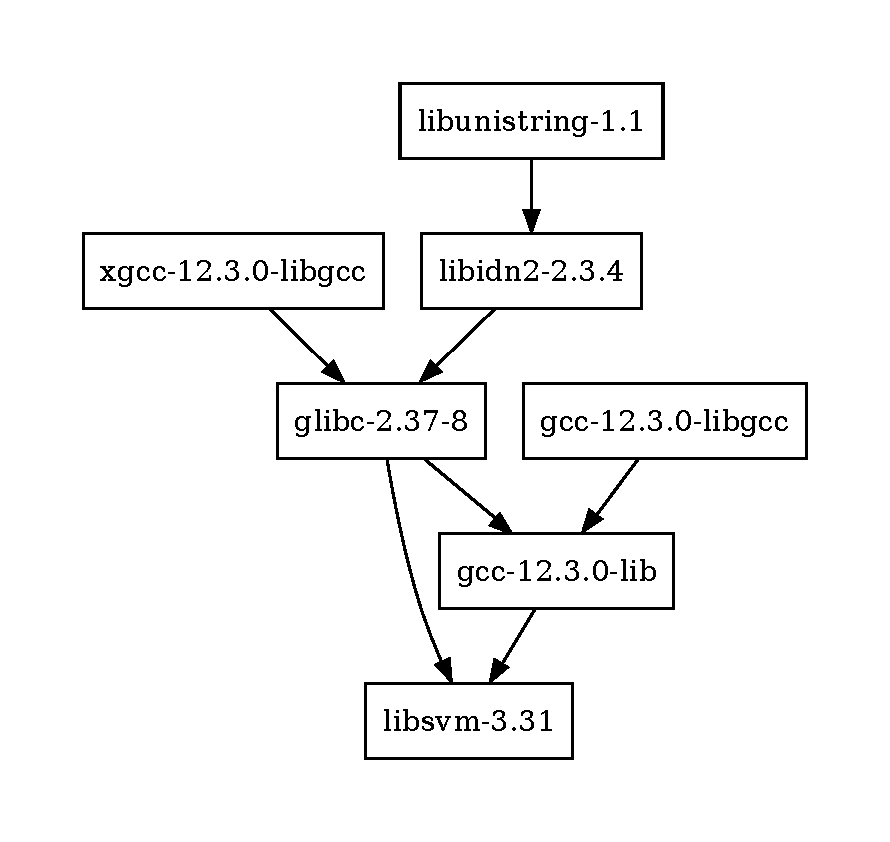
\includegraphics[width=.95\linewidth]{dependency_tree_libsvm}
    \caption{\emph{libsvm} runtime dependencies.}
    \label{fig:dependency_tree_libsvm}
\end{wrapfigure}

To manage the dependencies of the project, we use \emph{nix}
\cite{NixNixOSReproducible}, a purely functional package manager. \emph{Nix}
allows us to keep a consistent environment across different machines and
operating systems. It keeps track of \emph{all} the system dependencies of the
project including all the libraries and tools (such as compilers, interpreters,
etc.). For instance, with \emph{nix} we can visualize the runtime dependency
tree of the \emph{libsvm} library as shown in \cref{fig:dependency_tree_libsvm}.

On the \emph{Julia} side, the dependencies are managed through \emph{Pkg}
\cite{PkgJuliaLanguage}. All this complexity is hidden from the user through
\emph{direnv} \cite{DirenvUnclutterYoura}, which automatically loads the
environment when entering the project directory.

In summary, to reproduce the exact environment in which the experiments were
run, the user only needs to install \emph{nix} and \emph{direnv} and run
\texttt{direnv allow} in the project directory.

All the datasets used are publicly available and are downloaded automatically by
\emph{nix}. There is a file \texttt{datasets.toml} which contains the URLs of
the datasets and their checksums\footnote{The checksum uses
    \url{https://www.mankier.com/1/nix-hash}}, this guarantees that other users will
know if the dataset has been modified.

\begin{listing}[htpb]
    \caption{Fragment of the \texttt{datasets.toml} file.}
    \label{lst:datasets_toml}
    \inputminted[firstline=29,lastline=35]{toml}{../datasets.toml}
\end{listing}

\subsection{Build system}

To build the project, we use \emph{Nix} as well. The \emph{Nix} build system is
a declarative build system which allows us to specify the exact build steps and
dependencies of the project. Since the build steps are sandboxed with no access
to the system or the network, the build is guaranteed to be reproducible as long
as the process is deterministic (see \cref{sub:deterministic}).

\subsubsection{Determinism}
\label{sub:deterministic}

A deterministic build is a build that produces the same result given the same
inputs. There are many factors that can affect the result of a build, such as
the time of the build, the use of random numbers, race conditions, network
access, etc.

To mitigate these factors, where possible, we use a fixed seed for the random
number generator in \emph{Julia} and set the \texttt{SOURCE\_DATE\_EPOCH}
environment variable to a fixed date. The only factor that we do not control is
the execution order of different processes when running in parallel. However,
the multiple processes do not interact with each other in our case, so this
should not affect the result.

\subsection{Version control}

All versions of the code are stored in a \emph{git} repository hosted on GitHub.
% TODO: link to repo Additionally, all executions of experiments that generate
data, store the commit hash of the repository in which the code was run. This
allows us to trace back the exact version of the code used to generate the data.
This is handled through the \texttt{DrWatson.jl} package
\cite{datserisDrWatsonPerfectSidekick2020a}.

\subsection{Storing the results}

The \emph{DrWatson.jl} package also provides a mechanism to store the results of
the experiments, in which the results are serialized and stored in a \emph{JLD2}
file (a julia-specific version of the \emph{HDF5} format). Additionally, it
stores several metadata fields such as the commit hash, the parameters used and
other information such as the computed performance metric or any other relevant
information we may need. The filename for each result saved is generated from
the relevant parameters, which allows checking whether a certain parameter
configuration has already been computed and load it instead of recomputing it.

These \emph{JLD2} files contain the whole state of the trained machine models,
which is useful to be able to load the models and inspect them later. However,
this also means that the files are quite large (several hundred megabytes). For
most analysis we are only interested in the performance metric of the model, so
along with the \emph{JLD2} files, we also store a \emph{CSV} file with the
relevant information for each model. This allows us to quickly load the results
and perform analysis on them and, if necessary, we can load the full model from
the \emph{JLD2} file. This workflow is illustrated in
\cref{fig:experiment_flowchart}.

\begin{figure}[H]
    \begin{tikzpicture}
        % card with bullet points
        \node[draw, rectangle, minimum width=5cm, minimum height=3cm] (card) at (0,0) {};
        \node[anchor=north west] at (card.north west) {\textbf{Experiment\_1}};
        \node[anchor=north west] at ($(card.north west)+(0.2,-0.5)$) {- \texttt{sigma} = 0.1};
        \node[anchor=north west] at ($(card.north west)+(0.2,-1)$) {- \texttt{epsilon} = 0.5};
        \node[anchor=north west] at ($(card.north west)+(0.2,-1.5)$) {- \texttt{kernel} = \texttt{ArcSin}};
        \node[anchor=north west] at ($(card.north west)+(0.2,-2)$) {- \texttt{dataset} = \texttt{Triazines}};
        \node[anchor=north west] at ($(card.north west)+(0.4,-2.5)$) {\dots};

        \node (name) [below=of card] {\texttt{ex1\_sigma=0.1\_epsilon=0.5}\dots\texttt{.jld2}};
        \draw[-] (card) -- (name) node[midway, anchor=west] { filename};

        % if file exists, else

        \node[draw, diamond] (if) [below=of name] {Exists?};
        \draw[->] (name) -- (if);
        \node[draw, rectangle, rounded corners, inner sep = 10pt] (load) [left =of if] {Load};
        \node[draw, rectangle, rounded corners, inner sep = 10pt] (run) [right=of if] {Run};
        \draw[->] (if) -- (load) node[midway, anchor=south] {yes};
        \draw[->] (if) -- (run) node[midway, anchor=south ] {no};

        \coordinate [right=of name] (nameright) {};
        \node (csv) [right=of nameright] {\texttt{ex1\_results.csv}};

        \draw[-] (run.east) -| (nameright) node[midway, anchor=south west] {save};
        \draw[->] (nameright) |- (name);

        \draw[->] (run.east) -| (csv.south) node[midway, anchor=south west] {append};
    \end{tikzpicture}
    \caption{Flowchart of the experiment execution and results storage.}
    \label{fig:experiment_flowchart}
\end{figure}

\subsection{Running the experiments}

All the relevant code to the experiments is contained in the \texttt{src}
directory and scripts that run the experiments are in the \texttt{scripts}
directory and named after their corresponding experiment. To run an experiment,
we can simply call the corresponding \emph{Julia} script:
\mintinline{bash}{julia scripts/experiment_1.jl}. The dependencies can be
installed automatically using \emph{Nix} and \emph{direnv} as described in
\cref{sub:dependency_management}, with \mintinline{bash}{direnv allow} or
\mintinline{bash}{nix develop}.

Additionally, the \mintinline{bash}{nix build} command can be used to build the
document and a tarball with the datasets.

\section{Extending \texttt{libsvm}}%
\label{sub:impl_c}

\emph{libsvm} is a C library developed by \textcite{CC01a} under BSD-3 license
which implements the Support Vector Machine (SVM) algorithm. The library is the
de facto standard for SVM implementations in the machine learning community,
being used by many other libraries and frameworks such as Python's
sklearn~\cite{ScikitlearnScikitlearn2023} or R's
e1071~\cite{meyer[autE1071MiscFunctions2023}.

Out of the box, \emph{libsvm} supports using the built-in kernels: linear,
polynomial, radial basis function (RBF) and sigmoid. Additionally, it can use
precomputed kernel matrices by setting the kernel type to \texttt{PRECOMPUTED}
and passing the kernel matrix as the training data.

The use of precomputed kernel matrices allows us to use any kernel function
of our choice. However, this requires computing the kernel matrix in advance,
which is not feasible for large datasets, since it requires $O(n^2)$ memory and
$O(n^2d)$ time, where $n$ is the number of samples and $d$ is the number of
features.
Instead, we can extend the library to add our own kernel functions
and let \texttt{libsvm} compute the values as needed.
The \texttt{libsvm} library is quite efficient in caching the kernel evaluations
and since it uses a Sequential Minimal Optimization algorithm, it only requires
some columns of the kernel matrix at a time \cite{CC01a}.

\subsection{Adding the kernels}

For our purposes, we want to extend the library by adding our own kernels. To do
so, we need to modify the library source by adding the corresponding kernel
functions. The kernel type is specified through an \texttt{enum}, so we can add
our own kernels to it and extend the switch statements in the code to handle
them. The modification is thus quite straightforward.
\cite{arquemartinezDissenyImplementacioEstudi2021}

From there, we have to implement the kernel functions themselves. Surprisingly
at first, the kernel functions are duplicated in the code for each kernel type:
\texttt{k\_function} and \texttt{kernel\_function}. The former is used for the
training phase and the latter for the prediction phase. This is explained in the
\emph{libsvm}'s FAQ \cite{LIBSVMFAQ}:

For the RBF kernel, Instead of doing $\exp\left(-\gamma\|x_i - x_j\|^2\right)$,
it computes $\exp\bigl(-\gamma(\|x_i\|^2 - 2x_i^Tx_j + \|x_j\|^2)\bigr)$, and by
precomputing $\|x_i\|^2$ for all $x_i$ in the beginning, the number of
operations is reduced from $3n$ to $2n$. This same optimization can be applied
to our kernels. \Cref{fig:c_improvement} shows the improvement in performance
when using this optimization.

% \begin{cnote}
%     The plot probably should be improved:
%     Better legend, change labels and remove RBF since it is not relevant.
%     Also, add error bars?
% \end{cnote}
% TODO: Improve plot and explain better what is shown:
% - Better legend
% - Consistent colors with other kernel plots
% - probably make height smaller
\begin{figure}[H]
    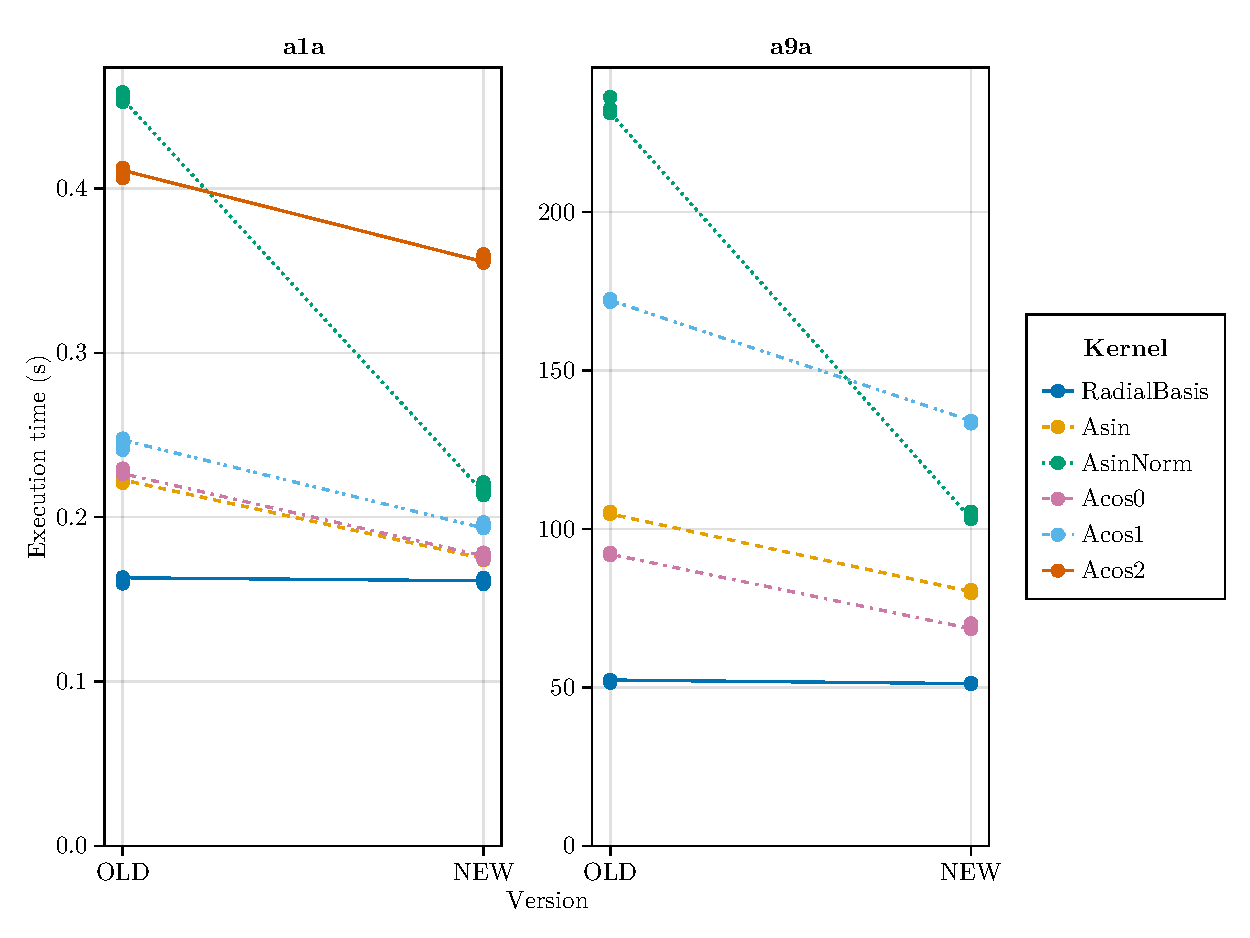
\includegraphics{plots/benchmark_time_improvement_old}
    \caption{Comparison between kernels on the training phase with and without
        pre-computation when training the Adult dataset}%
    \label{fig:c_improvement}
\end{figure}

The first step, is to add the new kernel types to the \texttt{enum} in
\texttt{svm.h} as shown in \cref{lst:svm_h_enum}.
\begin{listing}[H]
    \caption{Modified Enum definition from \texttt{svm.h}}
    \label{lst:svm_h_enum}
    \begin{minted}{C}
enum { LINEAR, POLY, RBF, SIGMOID, PRECOMPUTED, ASIN, ASIN_NORM, ACOS_0, ACOS_1, ACOS_2}; /* kernel_type */
\end{minted}
\end{listing}
Then, we add the corresponding cases to the switch statements in
\texttt{svm.cpp} for both \texttt{k\_function} and \texttt{kernel\_function} as
shown in \cref{lst:kernel_function}. The prediction case (\texttt{k\_function})
is not shown for brevity, but it is similar to the training case. The only
difference is the use of the precomputed dot product of $x_i$ with itself
(\texttt{x\_square}), which is passed as a parameter to the kernel function (See
\cref{lst:svm_cpp_k_function} in the appendix)

In order to avoid code duplication and make the code more readable, we added the
helper functions for the \texttt{asin} kernel shown in
\cref{lst:svm_cpp_helper}.

Another minor optimization for the \texttt{asin} kernel, instead of computing
$\frac{1}{2\sigma_w^2}$ every time as shown in the original
\cref{eq:kernel_asin}, we define $\gamma = \frac{1}{2\sigma_w^2}$ and pass it as
a parameter to the kernel function.

\begin{listing}[H]
    \caption{Helper functions for the asin kernel (\texttt{svm.cpp})}
    \label{lst:svm_cpp_helper}
    \begin{minted}{C}
// Passing x_square and y_square as parameters, we can avoid computing them again
// every time we call the kernel function
static inline double asin_elm(const svm_node *x, const svm_node *y, const double x_square, const double y_square, const double gamma) {
    return asin((1.0 + dot(x, y))/sqrt( (gamma + 1.0 + x_square)* (gamma + 1.0 + y_square)) );
};

// Fallback method used in prediction
static inline double asin_elm(const svm_node *x, const svm_node *y, const double gamma) {
    return asin_elm(x, y, dot(x), dot(y), gamma);
}

// AsinELM with x=y, for faster computation, we don't need to compute the sqrt
static inline double asin_elm_equal(const double x_square, const double gamma) {
    const double x_square_plus_one = 1.0 + x_square;
    return asin(x_square_plus_one/(gamma + x_square_plus_one));
}
\end{minted}
\end{listing}

\begin{listing}
    \caption{Implementation of the kernels in \texttt{svm.cpp} for the training phase. \\[0.5em]
        (Notice the use of \texttt{x\_square} to avoid computing the dot product of $x$ with itself every time)
    }
    \label{lst:kernel_function}
    \begin{minted}{C}
double kernel_asin(int i, int j) const
{
    return M_2_PI*asin_elm(x[i], x[j], x_square[i], x_square[j], gamma);
}
double kernel_asin_norm(int i, int j) const
{
    return asin_elm(x[i], x[j], x_square[i], x_square[j], gamma)/sqrt(
        asin_elm_equal(x_square[i], gamma)*asin_elm_equal(x_square[j], gamma)
    );
}
double kernel_acos_0(int i, int j) const
{
    return 1.0 - M_1_PI*acos(dot(x[i], x[j])/sqrt(x_square[i]*x_square[j]));
}
double kernel_acos_1(int i, int j) const
{
    const double x2y2 = x_square[i]*x_square[j];
    const double xy = sqrt(x2y2);
    const double cos_theta = dot(x[i], x[j])/xy;
    const double theta = acos(cos_theta);
    return M_1_PI*xy*(sin(theta) + (M_PI - theta)*cos_theta);
}
double kernel_acos_2(int i, int j) const
{
    const double x2y2 = x_square[i]*x_square[j];
    const double sqrt_x2y2 = sqrt(x2y2);
    const double dot_xy = dot(x[i], x[j]);
    const double cos_theta = dot_xy/sqrt_x2y2;
    const double cos2_theta = dot_xy*dot_xy/x2y2;
    const double theta = acos(cos_theta);
    return M_1_PI*x2y2*(3*sin(theta)*cos_theta + (M_PI - theta)*(1 + 2*cos2_theta));
}
\end{minted}
\end{listing}

\subsection{Controlling the number of iterations}

One metric which we wanted to measure was the number of iterations the SVM
algorithm took and have the possibility to stop it early. To do so,
\emph{libsvm} only provides a \texttt{tolerance} parameter for the stopping
criterion. However, in \emph{sklearn} they provide a \texttt{max\_iter}
parameter\footnote{\url{https://github.com/scikit-learn/scikit-learn/pull/1184}}
which is the maximum number of iterations and also report the number of
iterations the algorithm took
\footnote{\url{https://github.com/scikit-learn/scikit-learn/pull/21408}}. This
is accomplished by using a modified version of \emph{libsvm}. Since we are
modifying the library as well, we added the same functionality to our modified
version

\pagebreak % INFO: make sure this is start of page so wrapfigure plays nice
\section{Julia}%
\label{sub:impl_julia}

\begin{wrapfigure}{r}{.40\textwidth}
    
\includegraphics[width=.95\linewidth]{julia-logo-color}
    \caption{Julia logo.\protect\footnotemark}
    \label{fig:julia_logo}
\end{wrapfigure}
\footnotetext{Official Julia logo by Stefan Karpinski, licensed under \href{https://creativecommons.org/licenses/by-sa/4.0/}{CC BY-SA 4.0}.}

\emph{Julia} \cite{bezanson2017julia} is a high-level, high-performance dynamic
programming language which is designed from the ground up to be fast,
expressive, and easy to write. Its aim is to provide the ease of use of a
scripting language such as Python while being as fast as a compiled language
such as C. In particular, \emph{BinaryBuilder.jl}
\cite{JLLPackagesBinaryBuilder} allows reproducible cross-platform compilation
of 3rd party libraries for different platforms and architectures. This is used
throughout the Julia ecosystem to provide binary dependencies for packages, for
example, \emph{libsvm} is provided by the \emph{libsvm\_jll} package
\cite{LibsvmJllJl2022}. This makes it very easy to change the \emph{libsvm}
library used by a package by simply changing the dependency to our modified
\emph{libsvm\_jll} package.

The latest stable version at the time of writing (1.9.x) introduced a major
improvement on the time to first execution, which historically has been one of
the main drawbacks of the language. In previous versions, every new session had
to pre-compile all the libraries as they were loaded, which often could take
minutes. Now, this is cached between sessions\cite{JuliaV1Release}.

For the above reasons, along with the fact that there is a large and growing
number of machine learning packages in Julia, we decided to interface our
modified \emph{libsvm} library with Julia.

\subsection{libsvm\_jll}

As mentioned before, the \emph{libsvm\_jll} package is a compiled version of the
\emph{libsvm} C library compiled through \emph{BinaryBuilder.jl}. This so-called
\emph{Julia Link Library} (JLL) package is not much different from a regular
system library, except that its dependencies are dynamically linked to other JLL
packages.

For our implementation, we used the original recipe from
\textcite{LibsvmJllJl2022} and modified it to use our modified \emph{libsvm}
source code.

\subsection{LIBSVM.jl}

The \emph{LIBSVM.jl} package \cite{LIBSVMJl2023} is a Julia wrapper for the
\emph{libsvm} library which provides a high-level interface to the library. It
uses the artifacts generated by the \emph{libsvm\_jll} package and provides the
translation between Julia types and the C types used by the library.

\subsubsection{Adding the kernels}

The kernels can be added by extending the \texttt{Kernel} \texttt{enum} in Julia
to reflect the \texttt{enum} in the C library.
\begin{listing}[H]
    \begin{minted}{julia}
module kernel
@enum KERNEL Linear Polynomial RadialBasis Sigmoid Precomputed Asin AsinNorm Acos0 Acos1 Acos2
end
\end{minted}
    \caption{Julia \texttt{enum} definition for the kernels, equivalent to the C definition in \cref{lst:svm_h_enum}.}
    \label{lst:kernel_enum_julia}
\end{listing}

Technically, this is the only change needed to add the kernels to the library,
since the \emph{C} library has the kernel functions implemented and selects them
based on the kernel type enum.

\subsubsection{Adding the number of iterations}

The modification of the number of iterations is a little more involved and
requires modifying the \texttt{SVMModel} and \texttt{SVMParameter} types to
store the number of iterations as well as properly copying the values from the C
pointer into Julia object. In order to test that this was properly implemented,
we added a test set to \emph{LIBSVM.jl}. The tests validate that the number of
iterations copied from the C pointer is the same as the one returned by the
\emph{libsvm} library and that \texttt{max\_iter} is respected.

\subsubsection{libsvm 3.31}

The version of \emph{libsvm} used by \emph{LIBSVM.jl} is 3.25. It has not been
updated to the newest version 3.31, since it breaks the API by adding the option
of probability density estimation. Again, we worked around this by modifying the
library to properly handle the new API (this change will be upstreamed to
\emph{LIBSVM.jl}). % TODO: link to PR

\subsection{MLJ}

\emph{MLJ} \cite{blaomMLJJuliaPackage2020} is a machine learning framework for
Julia which provides a common interface for many machine learning packages. It
is the equivalent of \emph{scikit-learn} in Python. It provides an interface to
\emph{LIBSVM} through the \emph{MLJLIBSVMInterface.jl} package. By modifying
the latter package to include the \texttt{max\_iter} parameter, we can use it in
\emph{MLJ}.

From this point, we can use all the functionality provided by \emph{MLJ} to
train, evaluate, tune and visualize our SVM models with flexibility and ease.

\Cref{fig:julia_libsvm_deps} shows the relationship between the packages and how
the libraries interface with each other.

\begin{figure}[H]
    \begin{tikzpicture}[
            box/.style={draw, rectangle, minimum width=1cm, minimum height=1cm},
            C/.style={fill=wong_blue!40,postaction={pattern=north west lines,pattern color=wong_blue!10}},
            Julia/.style={fill=wong_green!70},
            JLL/.style={fill=wong_orange!70,postaction={pattern=north east lines,pattern color=wong_orange!10}},
        ]
        \node[box,C] (libsvm) at (0,0) {libsvm};
        \node[box,JLL,below=of libsvm] (libsvm_jll) {libsvm\_jll};
        \node[box,Julia,right=of libsvm_jll] (LIBSVM) {LIBSVM.jl};
        \node[box,Julia,right=of LIBSVM] (MLJLIBSVMInterface) {MLJLIBSVMInterface.jl};
        \node[box,Julia,below=of MLJLIBSVMInterface] (MLJ) {MLJ.jl};

        \draw[->] (libsvm) -- (libsvm_jll) node[midway, anchor=west,color=wong_green] {build\_tarballs.jl};
        \draw[->] (libsvm_jll) -- (LIBSVM);
        \draw[->] (LIBSVM) -- (MLJLIBSVMInterface);
        \draw[->] (MLJLIBSVMInterface) -- (MLJ);

        % Color Legend
        \matrix [draw,right] at ($(current bounding box.east)+(0.5,0)$) {
            \node [C,label=right:C] {};                    \\
            \node [JLL,label=right:Julia Link Library] {}; \\
            \node [Julia,label=right:Julia] {};            \\
        };

    \end{tikzpicture}
    \caption{Dependency graph of Julia packages exposing the libsvm library API.}
    \label{fig:julia_libsvm_deps}
\end{figure}

The forked versions of the libraries discussed in this section can be found in
the following repositories:
\begin{itemize}
    \item \url{https://github.com/LeixB/libsvm}
    \item \url{https://github.com/Leixb/build\_tarballs\_libsvm\_jll}
    \item \url{https://github.com/Leixb/libsvm\_jll.jl}
    \item \url{https://github.com/LeixB/LIBSVM.jl}
    \item \url{https://github.com/LeixB/MLJLIBSVMInterface.jl}
\end{itemize}

% \subsection{Memoization}
% TODO: Check if memoization if worth it or if we can do it manually in a more
% sensible way.

\subsection{Visualizing the kernels}

Once all the kernels are implemented and the \emph{Julia} interface through
\emph{MLJ} is also complete, we can try to run the kernels to produce some
plots and compare them with the equivalent plots from the literature.

\begin{figure}[H]
    \begin{subfigure}{.59\textwidth}
        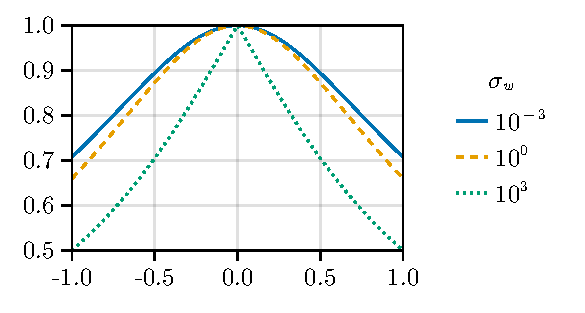
\includegraphics{plots/kernel_asin}
        \caption{Our custom implementation}
    \end{subfigure} \begin{subfigure}{.40\textwidth}
        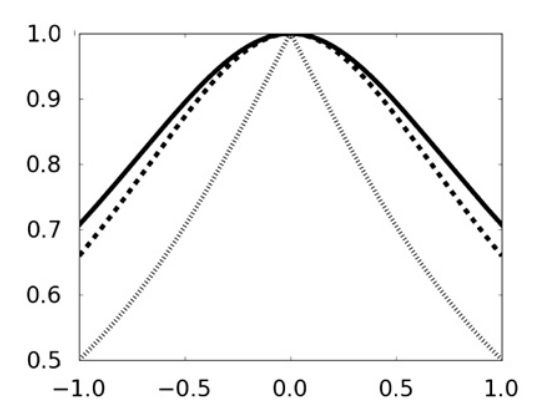
\includegraphics{frenay-kernel}
        \caption{\textcite{frenayParameterinsensitiveKernelExtreme2011}}
    \end{subfigure}
    \caption{Normalized Asymptotic ELM kernel evaluated around 0}
    \label{fig:kernel_asin_comparison}
\end{figure}

\Cref{fig:kernel_asin_comparison} shows the result of plotting the normalized
asymptotic ELM kernel around 0 through our implementation in \emph{Julia} and
the equivalent plot given in the original paper (the legend applies to both
plots).

\begin{cnote}
    Arc cosine kernels cannot be easily visualized in 2d, since 0 is undefined.
    Also, they look like their activation functions when plotted as done
    with asin.
\end{cnote}

% TODO: maybe add this?
% \subsection{Passing the kernel as a function pointer}
%
% One of the ideas explored was to instead of hard-coding the kernels in the
% library, set the kernel as a function pointer in libsvm. This would allow
% to define a function in Julia, get it's pointer and pass it to libsvm. This
% approach was evaluated and discarded since it would require a major
% refactor of the libsvm library and the divergence from the original library
% would make further updates more difficult.
%
% It is technically possible and worth exploring in the future, but the
% architecture of the libsvm library is quite constricted.


\section{Meta learning}
\label{sec:meta-learning}

The trial and error approach of machine learning tasks is often tedious and
time-consuming. Driven by this, multiple approaches have been proposed to make
recommender systems, which take the results of simple experiments and metrics
(meta-features) and use them to recommend hyperparameter values, search spaces
and optimization algorithms for similar tasks. This process of using
meta-features is a form of meta-learning. \Textcite{rivolliMetafeaturesMetalearning2022}
provides a comprehensive survey of the different meta-features and meta-learning
approaches.

\begin{important}
    Add table with meta-features (probably in appendix? There are 60+)
\end{important}
\begin{description}
    % TODO: probably rewrite all this descriptions
    % TODO: table with all the used meta-features? There are ~60
    \item[General]: also referred to as simple, are features that can be
    extracted from the data easily, with little computational cost. In this
    category, we have the number of instances, number of attributes, number
    of numeric attributes, the ratio of instances to attributes, etc.

    \item[Statistical]: as the name implies, they capture statistical properties
    of the data: mean, standard deviation, skewness, kurtosis, etc.
    These are only applicable to numeric attributes.

    \item[Information theory]: based on entropy measures, they capture the
    complexity and amount of information in the data.
    Only applicable to categorical attributes.

    \item[Model-based]: extracted from measures on models trained on the data.
    Usually from decision trees. These include the number of leaves, the
    number of nodes, the maximum depth, etc.

    \item[Landmarking]: not to be confused with the model-based, these focus
    on the performance of simple models on the data.
\end{description}

Implementing the meta-features and meta-learning algorithms is out of the scope
of this work, so we will use the \emph{PyMFE} python
package~\cite{WelcomePyMFEDocumentation,JMLR:v21:19-348} which provides
a vast collection of the most common meta-features.

Julia provides a convenient way to call Python code and libraries through the
\emph{PyCall.jl} package, which allows us to use \emph{PyMFE} from Julia, an
example of this is shown in \cref{lst:metafeatures}.

\begin{listing}
    \caption{Using \emph{PyMFE} from Julia to extract meta-features from a datasets.}%
    \label{lst:metafeatures}
    \begin{minted}{julia}
module MetaFeatures

import ..DataSets: DataSet, unpack
using PyCall, DataFrames, ProgressMeter

export extract_features

const MFE = pyimport("pymfe.mfe").MFE

"Return a Dict with the meta-features extracted from the dataset using the pymfe library."
function extract_features(X, y, args...; features=MFE.valid_metafeatures(), kwargs...)
    mfe = MFE(args...; features, kwargs...)
    mfe.fit(Matrix(X), y, precomp_groups=["general", "model-based", "landmarking"])
    ft = mfe.extract()

    # Convert list of tuples [(a, 7), (b, 4), ...] to Dict {a => 7, b => 4, ...}
    zip(ft...) |> Dict
end

function extract_features(datasets::Vector{<:DataSet}, args...; kwargs...)
    features = @showprogress map(datasets) do ds
        @info "Extracting features from $(ds)"
        X, y = unpack(ds)
        ft = extract_features(X, y, args...; kwargs...) |> DataFrame
        ft.dataset = [string(ds)]

        ft
    end

    vcat(features..., cols=:union)
end

end # module MetaFeatures
    \end{minted}
\end{listing}


% TODO: statistical meta-features we don't use since they take too long

\chapter{Experiments}
\label{sec:experiments}

Once the kernels are implemented, we can proceed to design and run the experiments using them.
We will follow the objectives and hypotheses stated in \cref{sec:objectives_and_hypotheses}. First
we outline the resampling strategy used in \cref{sec:resampling}, in \cref{sec:metrics} we
describe the metrics used to evaluate the performance of the kernels and in \cref{sec:datasets}
we describe the datasets used in the experiments.

\section{Common experimental setup}

\subsection{Resampling}

Instead of using the double cross-test resampling used in \cref{sec:reproducing-frenay},
we opted to use a 5\texttimes2 cross-validation resampling method as described by \textcite{dietterichApproximateStatisticalTests1998}.

The 5\texttimes2 cross-validation
consists of doing a 50\textendash50 split of the dataset into two sets. First, we train on the first set and test on the second set
and then we train on the second set and test on the first set. The process is repeated 5 times, each time
with a different random split. We choose this method since it is faster than the double cross-test method
requiring only 10 training processes instead of 100.

% TODO: Add figure of the 5-2 cross-validation ?

\subsection{Metrics}

For the metrics, we use the normalized root-mean-square error (\emph{nRMSE}), which is
a normalized version of the root-mean-square error (\emph{RMSE}) defined as follows:
\begin{equation}
    RMSE = \sqrt{\frac{1}{n}\sum_{i=1}^n (y_i - \hat{y}_i)^2}
\end{equation}

\subsection{Normalization}

In order to be able to compare the results between different datasets, an effort
was made to normalize the data and hyperparameters. To that end, the
following measures were implemented:

\begin{enumerate}
    \item Variables (including target) are standardized
    \item We use normalized root-mean-square error as our performance
        measure.
    \item The kernel itself is normalized.
    \item The hyperparameter $\sigma_w$ is divided by the number of samples in
        the training data of each dataset.
\end{enumerate}

In the next paragraphs we clarify how each of these steps are implemented and
what is their effect.

\paragraph{Variable Standardization} this is implemented by taking the mean and
standard derivation of each column of the training set and using it to
normalize the columns ($z_i = (x_i - \mu_i)/\sigma_i$). These values are saved as
part of the model and used again when running on the test set. This process
is also applied to the target variable.

This acts as a method of scaling the data to values that are well behaved
for the SVM.

\paragraph{Normalized Root-Mean-Square Error} We define the
normalized root mean square error (\emph{nRMSE}) as follows:

\begin{equation}
    nRMSE = \frac{RMSE}{\sigma_{obs}}
\end{equation}

\subsection{Parameter grid}

For the parameter search, we tried all the combinations of values
in the bounds show in \cref{tab:paramgrid} in a $\log 10$ scale with
spacing of factor of $10$ between values. For example, for $\sigma_w$ the values
were $10^{-3},\,10^{-2},\,\dots,\,10^{3}$
% TODO: write this part so that it is more clear?

\begin{table}[H]
    \caption{Bounds of parameter grid}%
    \label{tab:paramgrid}
    \begin{tabular}{ccc}
        \toprule
        Variable & lower & upper \\
        \midrule
        $\sigma_w$ & $10^{-3}$ & $10^3$ \\
        $\varepsilon$ & $10^{-5}$ & $10^1$ \\
        $C$ & $10^{-2}$ & $10^4$ \\
        \bottomrule
    \end{tabular}
\end{table}

\section{Reproducing the results of \texorpdfstring{\citeauthor{frenayParameterinsensitiveKernelExtreme2011}}{Frénay and Verleysen}}
\label{sec:reproducing-frenay}

The first objective is to reproduce the results obtained by \textcite{frenayParameterinsensitiveKernelExtreme2011},
which will help validate our implementation of the arc sine kernel, ensure that our experimental setup is
correct and to have a baseline to compare our results with. This also serves as a peer review
of their results.

In the paper, \citeauthor{frenayParameterinsensitiveKernelExtreme2011} use a double cross-test resampling
method which is illustrated in \cref{fig:frenay-cross-test}. First, they perform a 10-fold cross validation,
where the 9 folds of the training set are then used on a second 10-fold cross validation to determine the
best hyperparameters. This means that there are 100 training processes in total.

\begin{figure}[H]
    \begin{tikzpicture}[
		scale=0.66,
		every node/.style={font=\footnotesize},
	]
	% Draw main rectangle
	\def\nfolds{10}
	\pgfmathsetmacro{\trainfolds}{\nfolds-1}
	\pgfmathsetmacro{\splits}{\nfolds-2}
	\def\heightmult{0.5}

	\newcommand{\fold}[5]{%
		\draw[#2] #1 rectangle ($#1+(\heightmult*\trainfolds,1)$);
		% fill with pattern
		\filldraw[#3] ($#1+(\heightmult*\trainfolds,0)$) rectangle ($#1+(\heightmult*\nfolds,1)$);

		\draw ($#1+(\heightmult*\trainfolds/2,0)$) node[below,name=below-#5] {training set};
		\draw ($#1+(\heightmult*\nfolds,0.5)$) node[right,name=right-#5] {#4 set};

		% Draw vertical dashed lines for fold divisions
		\foreach \x in {1,...,\splits}{
				\draw ($#1+(\heightmult*\x,0)$) -- ($#1+({\heightmult*\x},1)$);
			}
	}

	\def\coltest{wong_blue}
	\def\colvali{wong_orange}

	\fill[shading=axis,top color=\coltest!40,bottom color=\colvali!40] (0,0) -- (\heightmult*\trainfolds,0) -- (\heightmult*\nfolds,-1) -- (0,-1) -- cycle;

	\fold{(0,0)}{fill=\coltest}{pattern=north east lines, pattern color=\coltest}{test}{test1}
	\fold{(0,-2)}{fill=\colvali}{pattern=north west lines,pattern color=\colvali}{validation}{val1}

	\draw[->] (0,0) -- (0,-1);
	\draw[->] (\heightmult*\trainfolds,0) -- (\heightmult*\nfolds,-1);

	% title above bounding box
	% \draw (current bounding box.north) node[above] {\textbf{Step 1: folding}};

	\fold{(9,0)}{fill=\colvali}{pattern=north west lines,pattern color=\colvali}{validation}{val2}

	\draw (right-val1.east -| below-val2.south) node[name=meta-parameters] {meta-parameters};
	\coordinate (a) at ($(meta-parameters)!.5!(below-val2)$);
	\node[name=model] at (a -| right-val2) {model};

	\coordinate (vm) at ($(model)!.5!(right-val2)$);
	\node[name=valerr] at ($(vm)+(5,0)$) {validation error};

	\coordinate (mm) at ($(meta-parameters.east |- model.west)!0.5!(model.west)$);
	\draw (below-val2.east) -| (mm);
	\draw (meta-parameters.east) -| (mm);
	\draw[->] (mm) -- (model);

	\coordinate (vvm) at ($(right-val2.east |- valerr.west)!0.5!(valerr.west)$);
	\draw (right-val2.east) -| (vvm);
	\draw (model.east) -| (vvm);
	\draw[->] (vvm) -- (valerr);

	% step 3

	\coordinate (step3) at (5,-5);
	\fold{(step3)}{fill=\coltest}{pattern=north east lines,pattern color=\coltest}{test}{test3}

	\draw ($(below-test3.south)+(0,-1)$) node[name=best-meta-parameters,text width=3cm,align=center]
	{best meta-parameters selected by cross-validation};

	\coordinate (b) at ($(best-meta-parameters)!.5!(below-test3)$);
	\node[name=model3] at ($(b -| right-test3)+(1,0)$) {model};

	\coordinate (vm3) at ($(model3)!.5!(right-test3)$);
	\node[name=testerr] at ($(vm3)+(5,0)$) {test error};

	\coordinate (mm3) at ($(best-meta-parameters.east |- model3.west)!0.5!(model3.west)$);
	\draw (below-test3.east) -| (mm3);
	\draw (best-meta-parameters.east) -| (mm3);
	\draw[->] (mm3) -- (model3);

	\coordinate (vvm3) at ($(right-test3.east |- testerr.west)!0.5!(testerr.west)$);
	\draw (right-test3.east) -| (vvm3);
	\draw (model3.east) -| (vvm3);
	\draw[->] (vvm3) -- (testerr);

	\coordinate (shift) at (0,1.5);
	\draw ($(0,0)+(shift)$) node[right] {\textbf{Step 1: folding}};
	\draw ($(9,0)+(shift)$) node[right] {\textbf{Step 2: meta-parameters selection on validation set}};
	\draw ($(step3)+(shift)$) node[right] {\textbf{Step 3: model assessment on test set}};

	% \draw ($(9,0)!0.5!(valerr.east) + (0,1.1)$) node[above] {\textbf{Step 2: meta-parameters selection on validation set}};

	% \draw ($(step3)!0.5!(step3 -| testerr.east) + (0,1)$) node[above] {\textbf{Step 3: model assessment on test set}};

\end{tikzpicture}

	\caption{Illustration of the cross-test method from \cite{frenayParameterinsensitiveKernelExtreme2011}}
	\label{fig:frenay-cross-test}
\end{figure}

\section{Comparing the performance of the kernels with different datasets}%
\sectionmark{Comparing performance}

\begin{figure}
    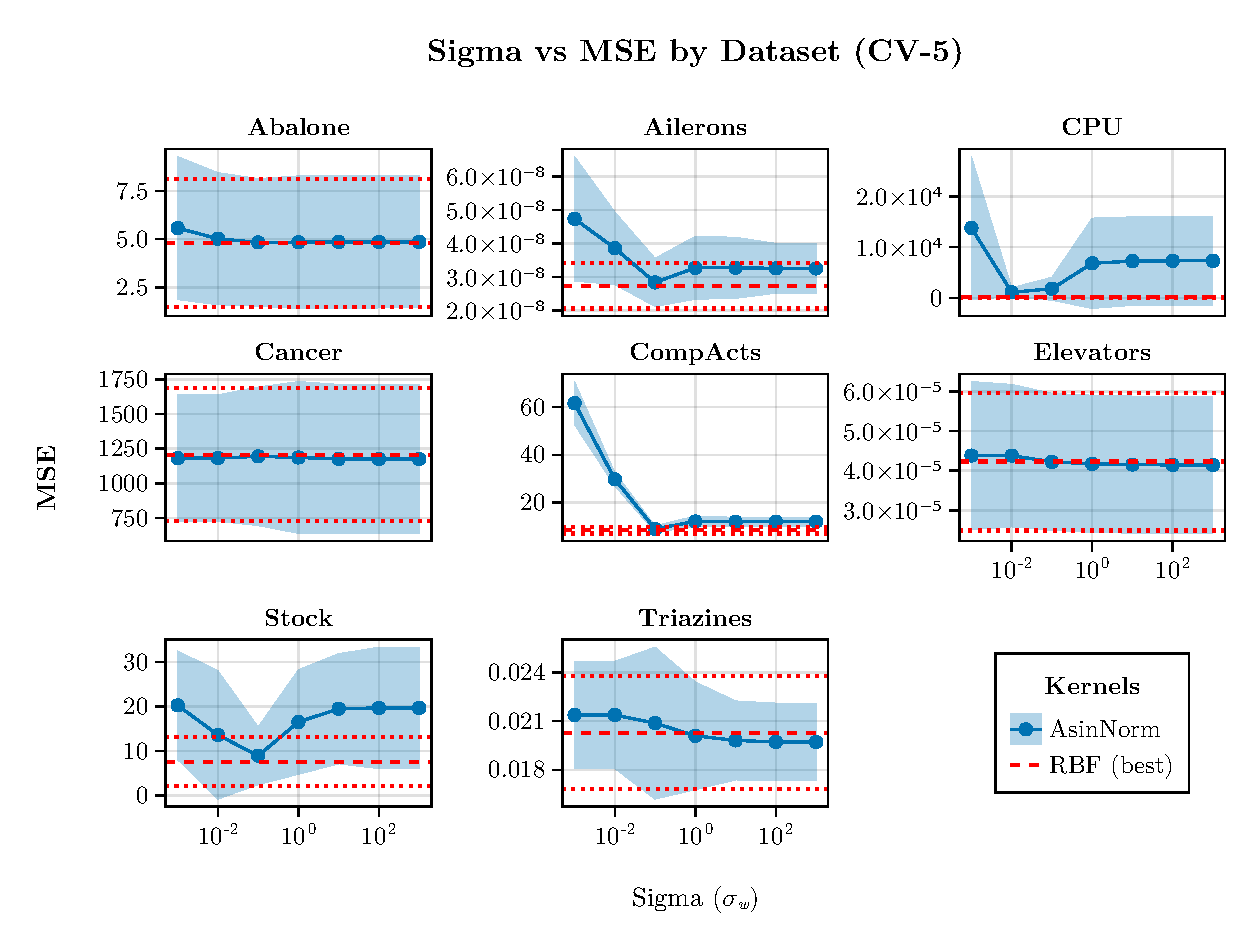
\includegraphics{plots/MSE_frenay}
    \caption{MSE results on datasets from \cite{frenayParameterinsensitiveKernelExtreme2011}}
\end{figure}


% NOTE: this is without scaling sigma
\begin{figure}
    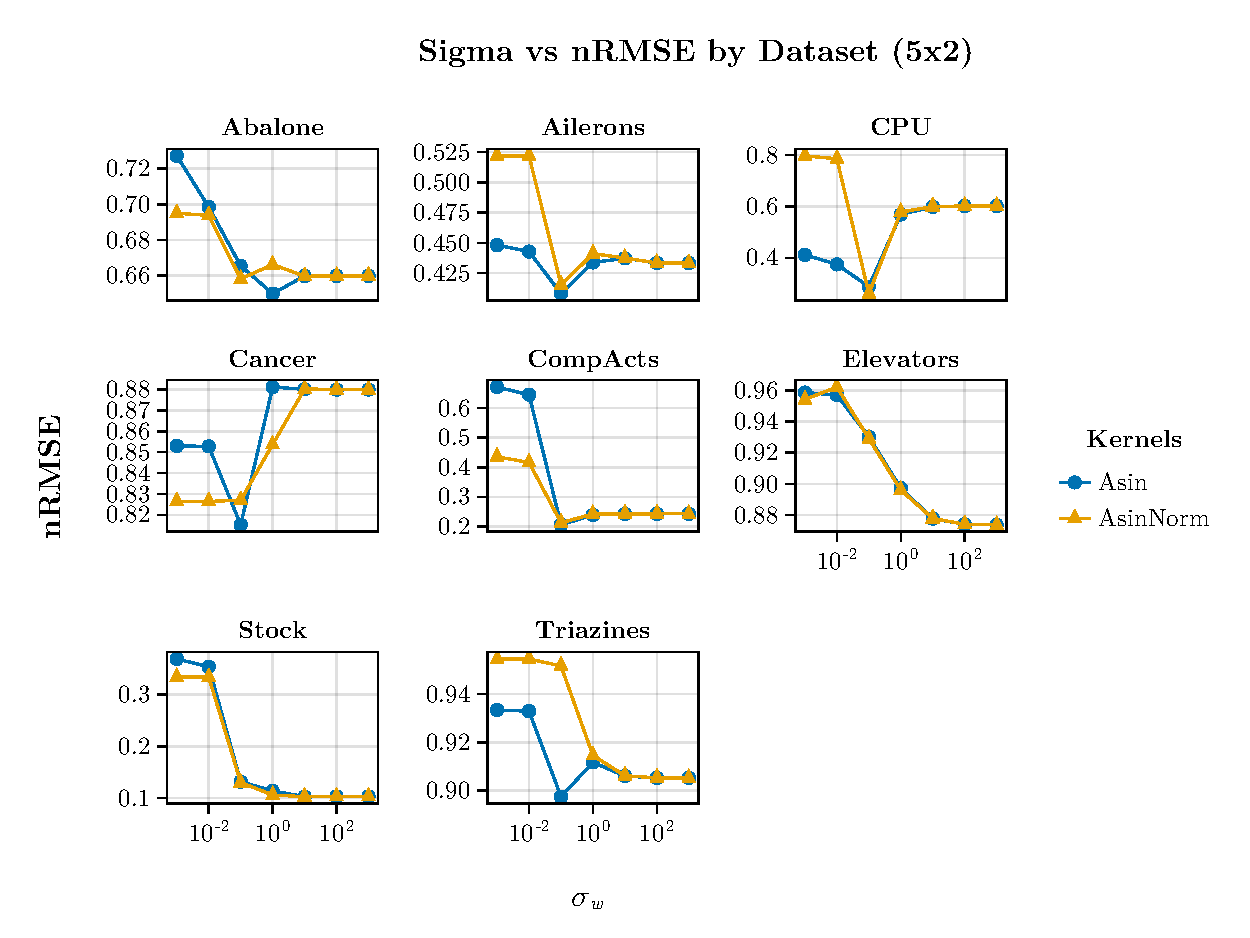
\includegraphics{plots/nRMSE_frenay}
    \caption{nRMSE results on datasets from \cite{frenayParameterinsensitiveKernelExtreme2011}}
\end{figure}

% WARN: these don't have all values of epsilon in our grid
\begin{figure}
    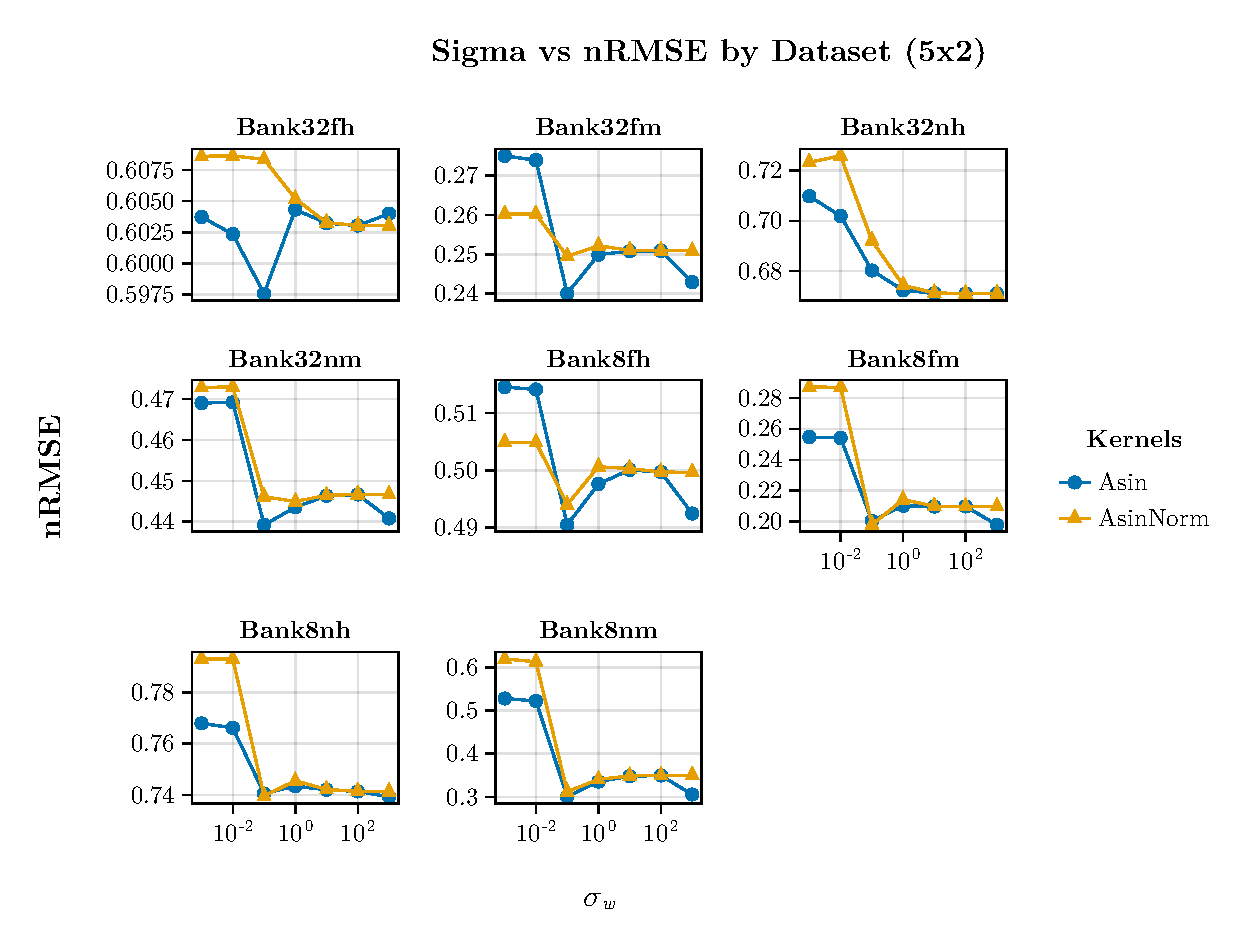
\includegraphics{plots/nRMSE_bank}
    \caption{nRMSE results on Delve Bank dataset}
\end{figure}

% WARN: these don't have all values of epsilon in our grid
\begin{figure}
    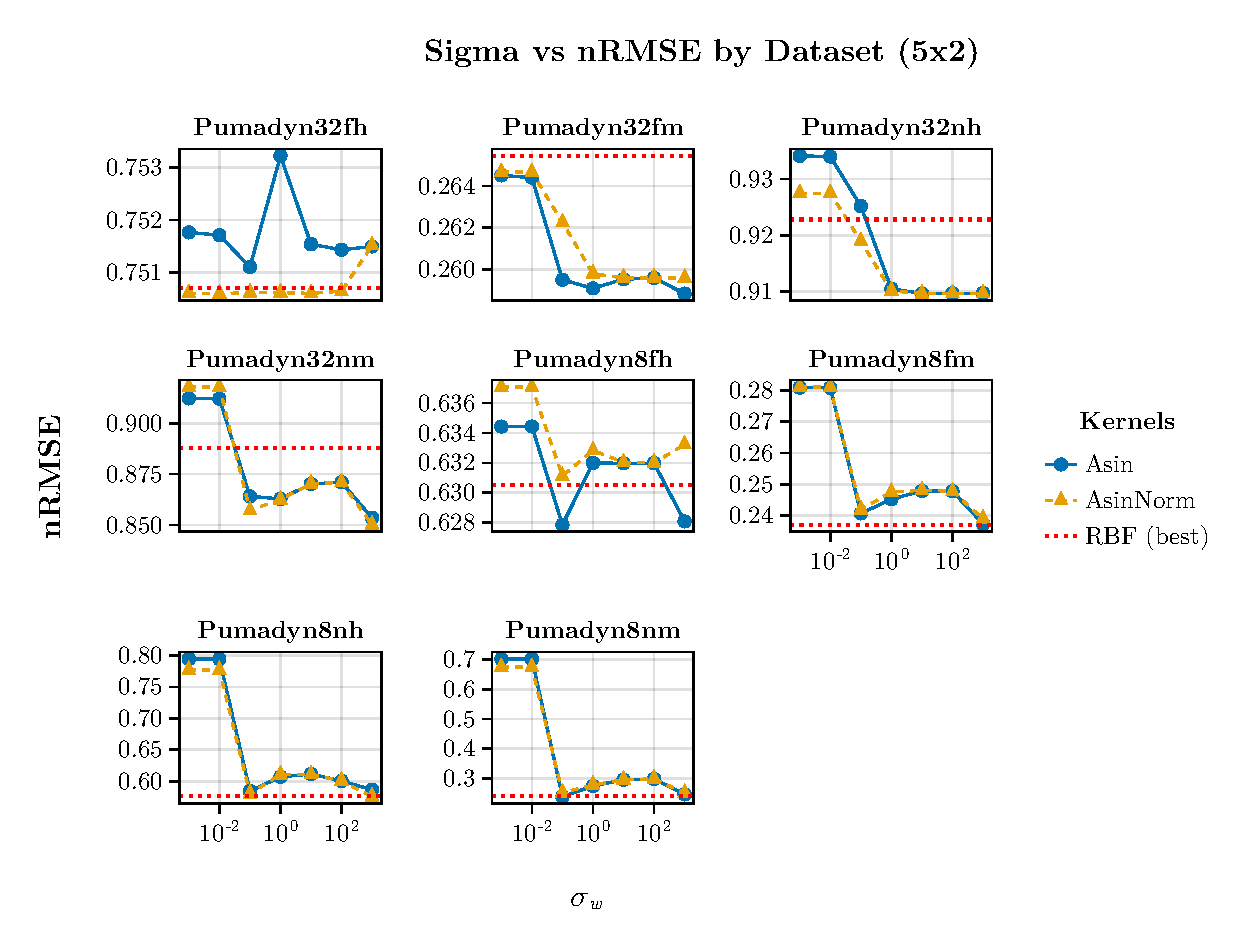
\includegraphics{plots/nRMSE_pumadyn}
    \caption{nRMSE results on Delve PumaDyn dataset}
\end{figure}

\begin{figure}
    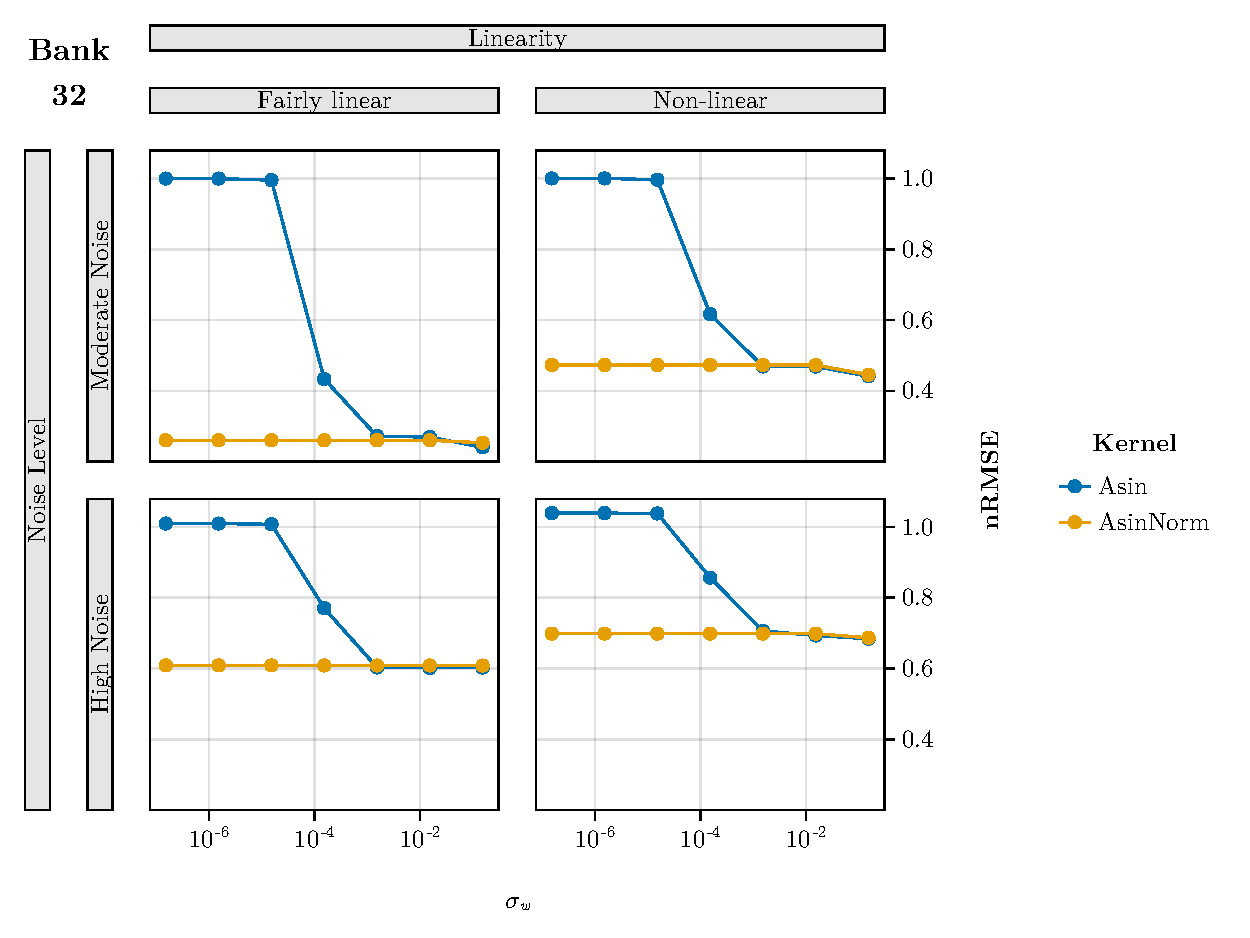
\includegraphics{plots/nRMSE_delve_bank_32_scaled}
    \caption{nRMSE results on Delve Bank32 dataset with $\sigma_w$ scaled}
\end{figure}

\begin{figure}
    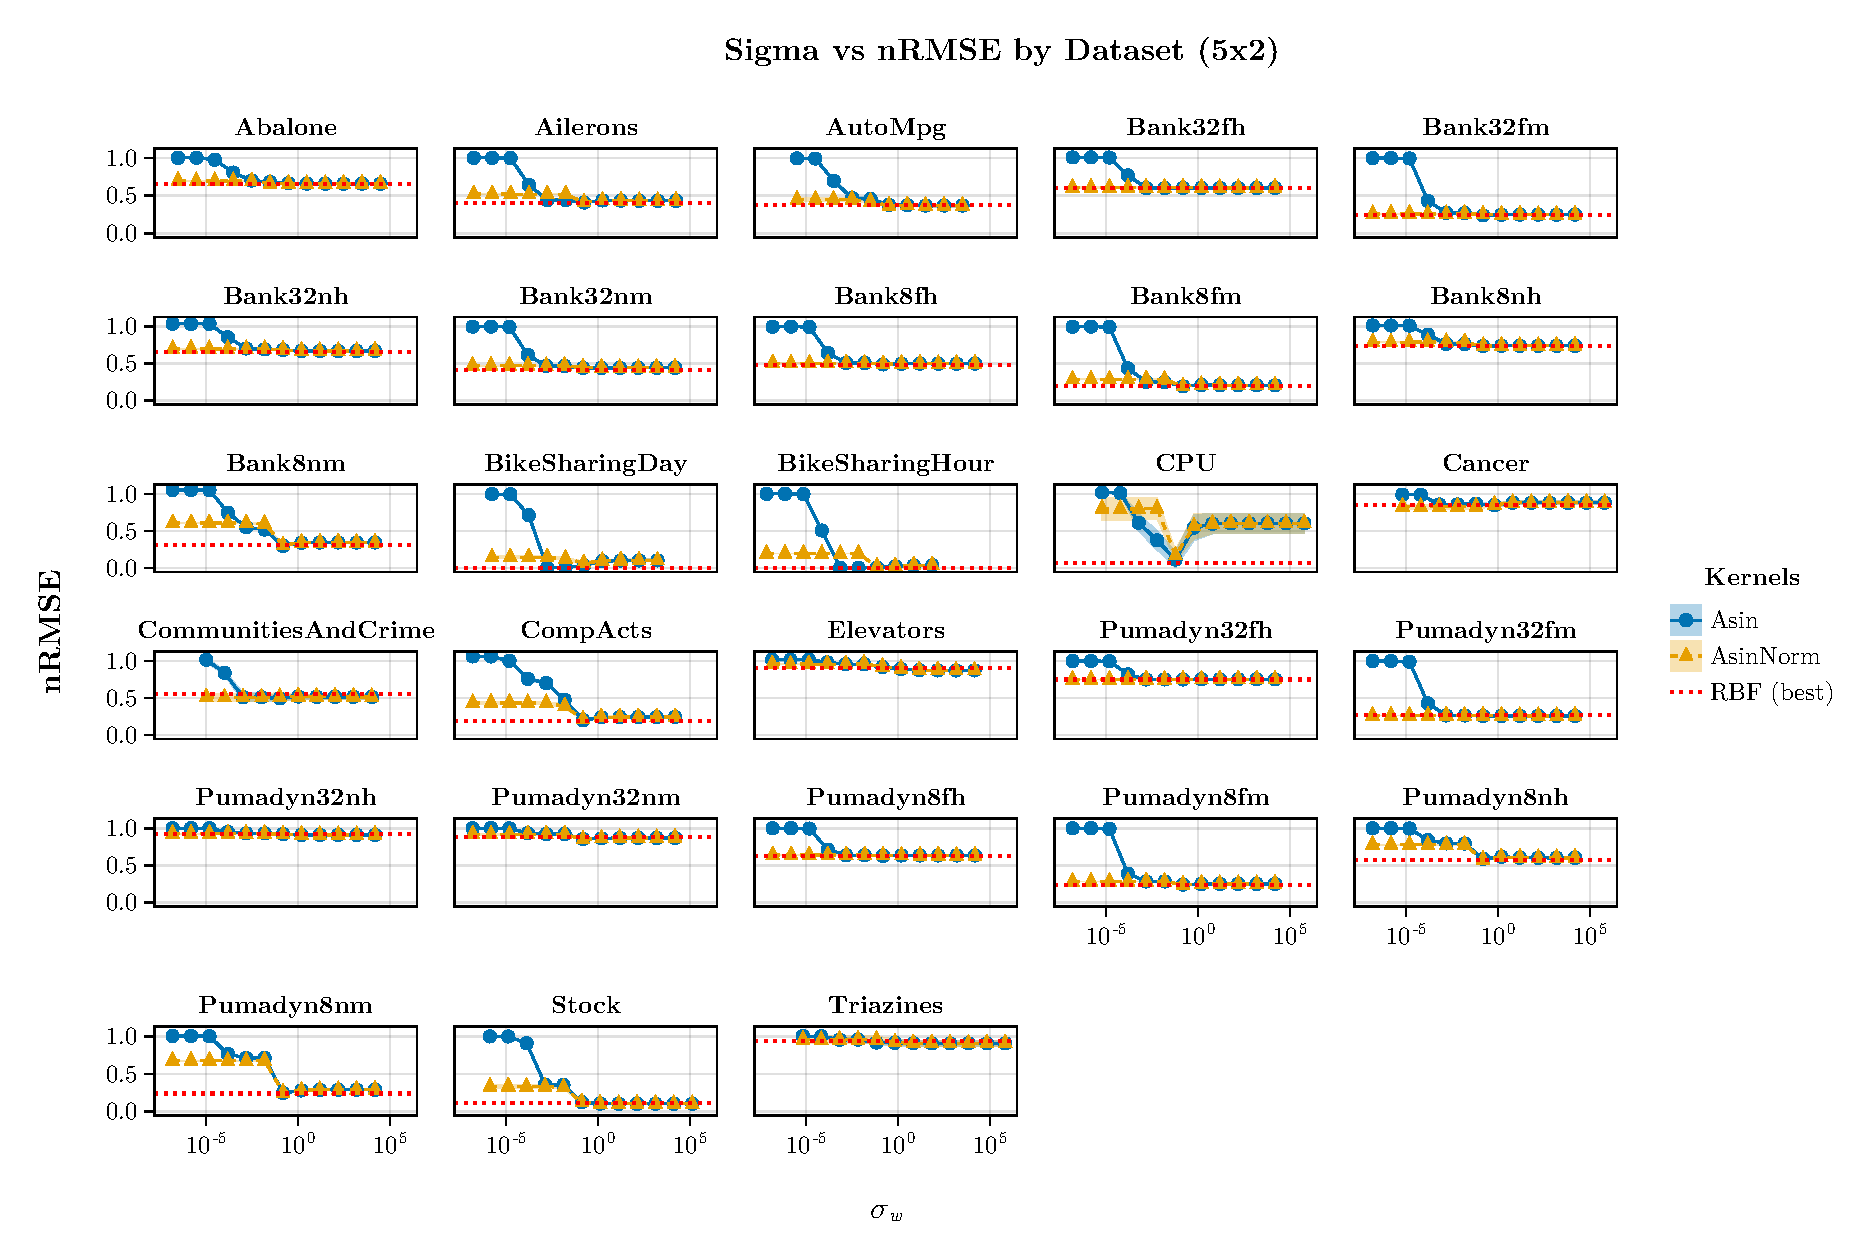
\includegraphics{plots/nRMSE_all_scaled}
    \caption{nRMSE results on Regression datasets with $\sigma_w$ scaled}
\end{figure}

\begin{figure}
    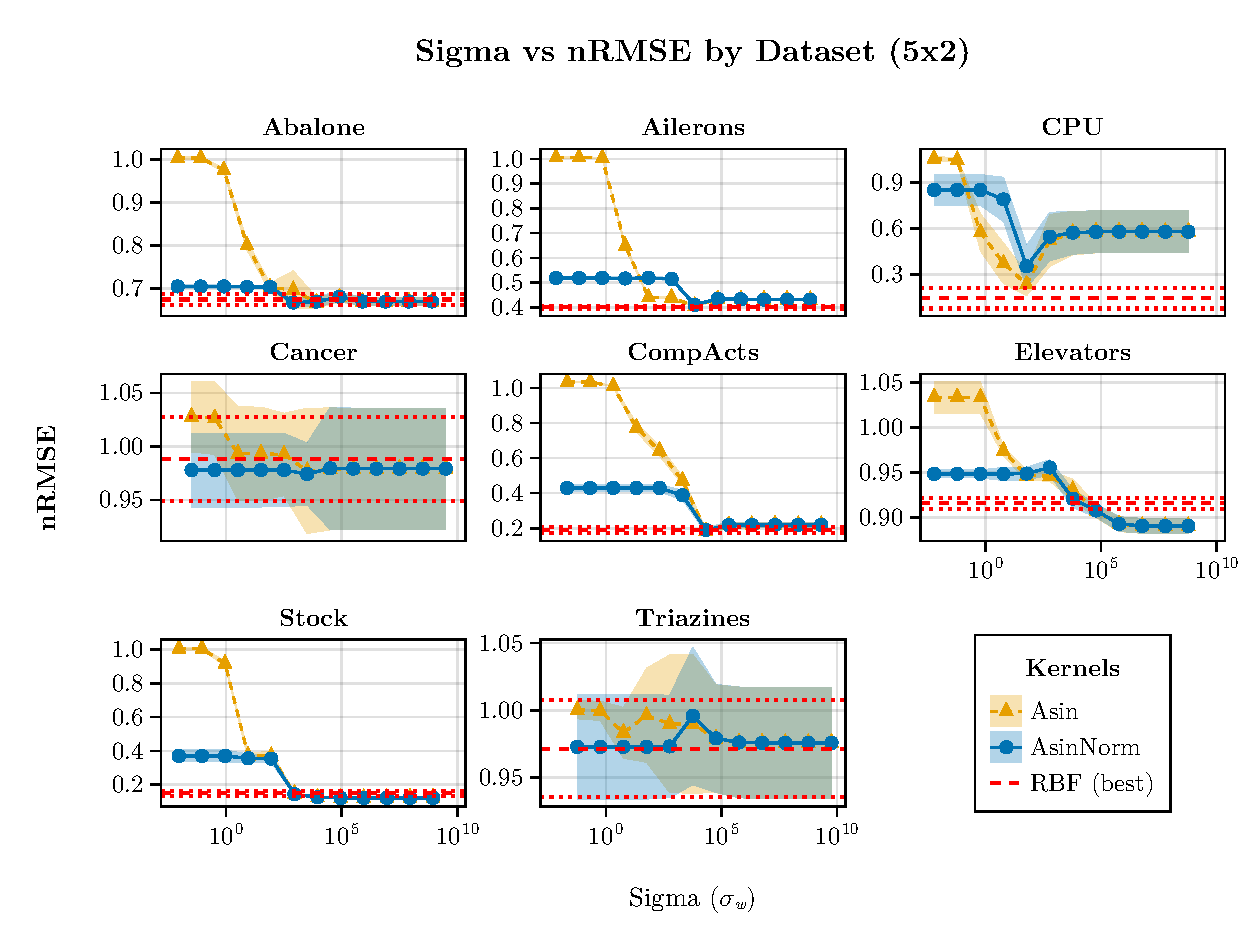
\includegraphics{plots/nRMSE_frenay_scaled}
    \caption{nRMSE results on Frenay datasets with $\sigma_w$ scaled}
\end{figure}

%! TEX root = **/000-main.tex
% vim: spell spelllang=en:
\chapter{Analysis}
\label{sec:analysis}

% 3d version
\begin{figure}
    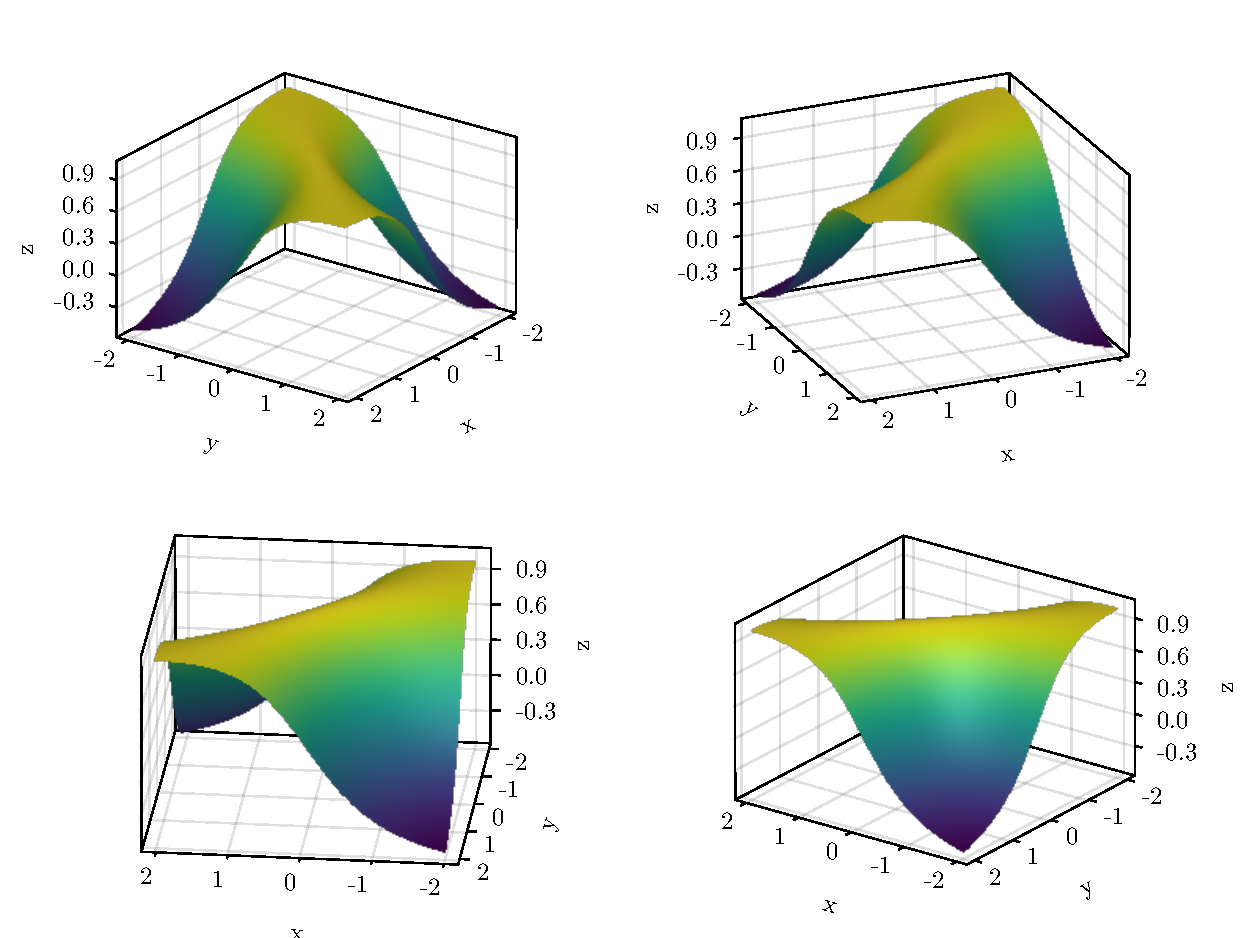
\includegraphics{plots/kernel_asin_3d_sig1}
    \caption{asin kernel with $\sigma_w=1$}
\end{figure}

\begin{figure}
    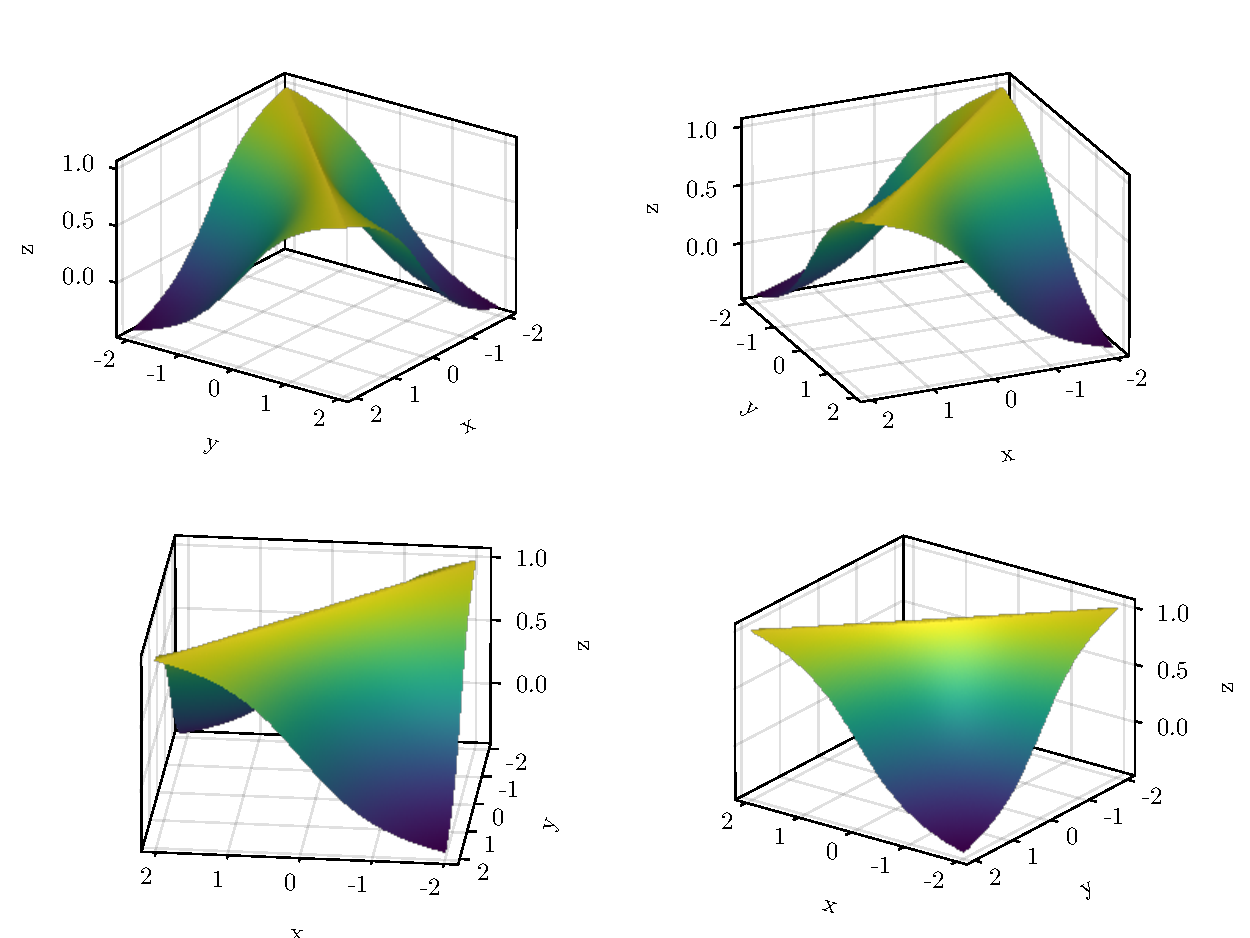
\includegraphics{plots/kernel_asin_3d_sig1000}
    \caption{asin kernel with $\sigma_w=1\,000$}
\end{figure}


% The acos ones are not very interesting with one dimensional vectors
\begin{figure}
    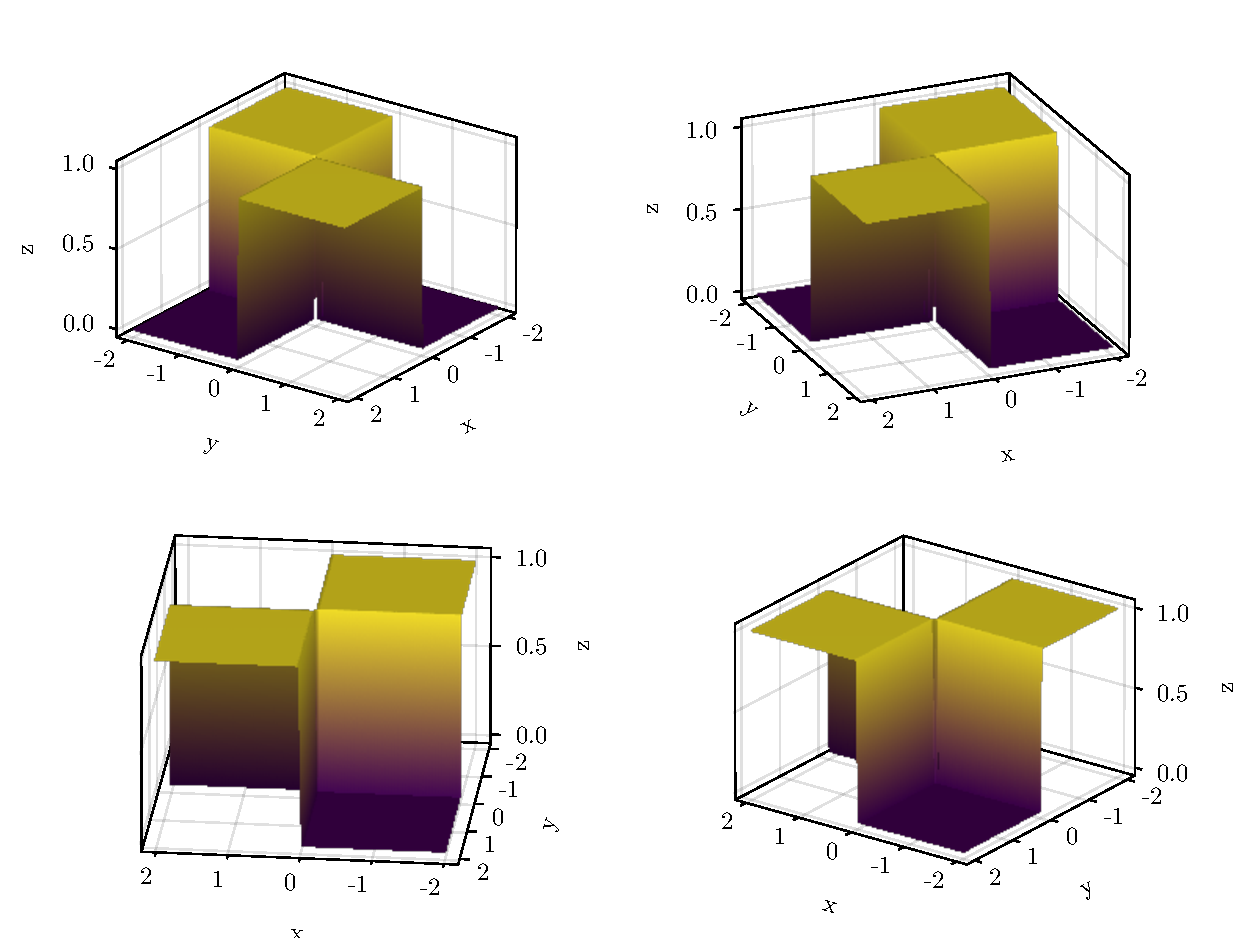
\includegraphics{plots/kernel_acos0_3d}
    \caption{acos kernel $n=0$}
\end{figure}

\begin{figure}
    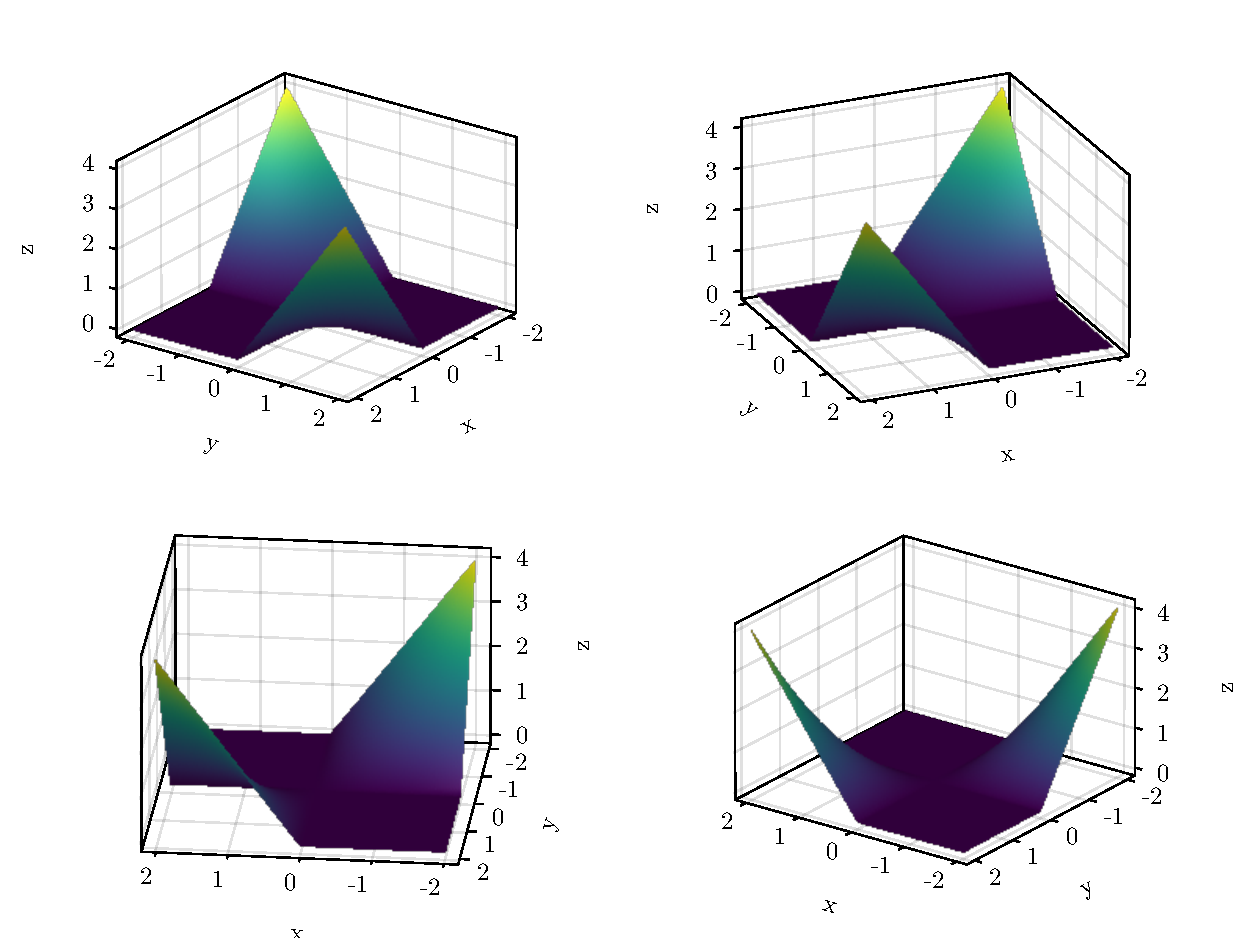
\includegraphics{plots/kernel_acos1_3d}
    \caption{acos kernel $n=1$}
\end{figure}

\begin{figure}
    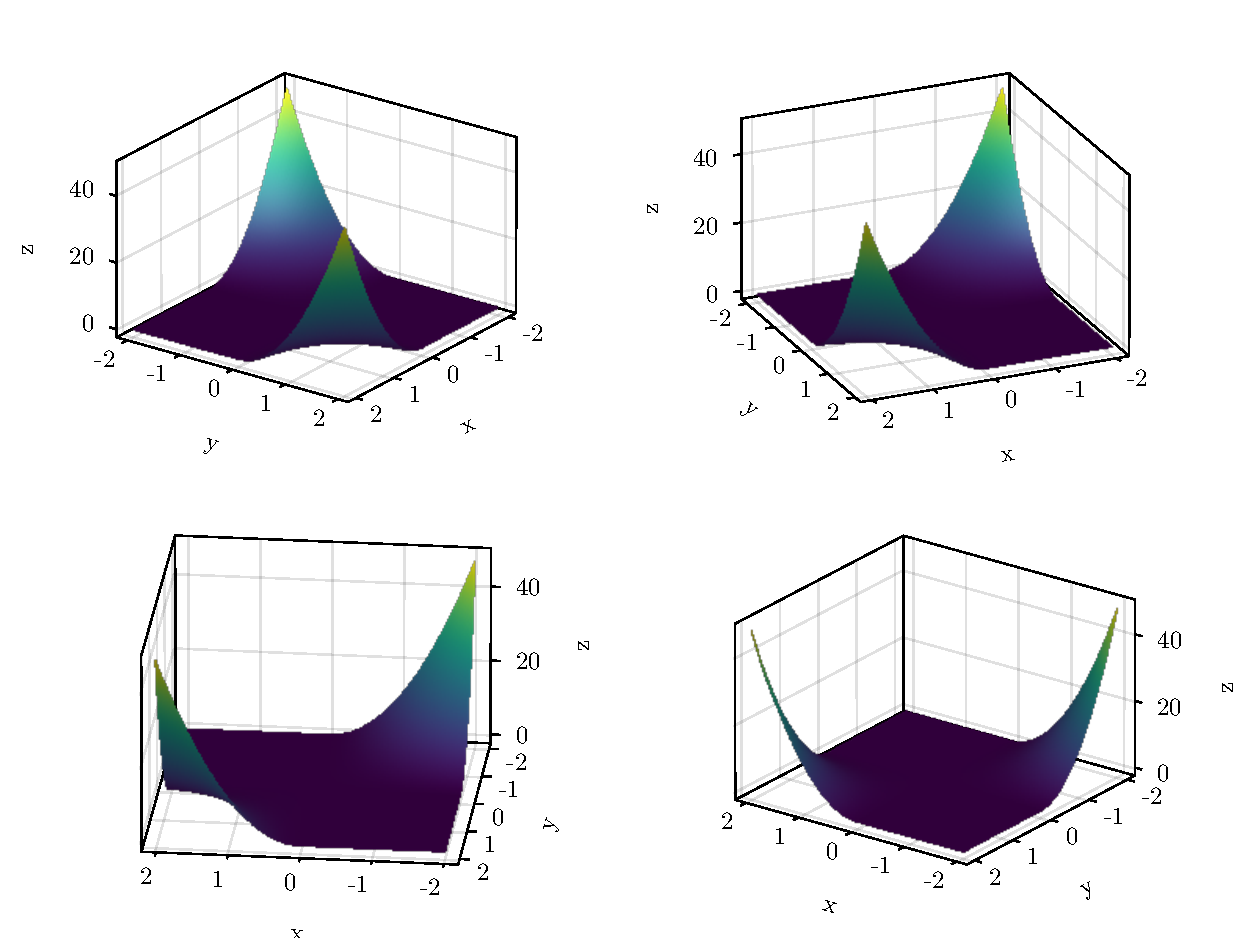
\includegraphics{plots/kernel_acos2_3d}
    \caption{acos kernel $n=2$}
\end{figure}

\chapter{Conclusions}
\label{sec:conclusions}

\section{Summary of results}

With this thesis we have explored the behaviour of inifinite neural network
kernels that have been proposed in the literature and which have an analytical
form. We have found that this family of kernels is quite small, with only
the arc sine (or ELM kernel from \cite{frenayParameterinsensitiveKernelExtreme2011})
and the arc cosine kernels (\cite{choLargemarginClassificationInfinite2010}) which
both build on the work of \textcite{williamsComputingInfiniteNetworks1996}.

For the arc sine kernel (or ELM), we have reproduced the results of \textcite{frenayParameterinsensitiveKernelExtreme2011}
and explored the behaviour in several other datasets. Doing so, we have found that
indeed it is parameter insensitive for sufficiently large values of $\sigma_w$,
however, in some datasets, by using other smaller values of $\sigma_w$ the performance
improved significantly. Meaning that some tuning of the hyperparameter is still
necessary if we want to obtain the best results in all cases.

Normalizing the arc sine kernel does improve its performance for small values
of $\sigma_w$, but for sufficiently large values of $\sigma_w$ ($>10$), the
effect of kernel normalization is negligible. We have shown using a paired
t-test that with an $\alpha=0.001$, the null hypothesis that the normalized
and non-normalized arc sine kernels perform the same cannot be rejected for
$\sigma_w > 10^6$.

For the arc cosine kernel, we have shown that for $n=0,1,2$, the normalization
of the kernel makes it insensitive to the value of $\sigma_w$. Moreover, not
normalizing the kernel leads to potential numerical issues due to the large
values the kernel gives when the difference between the features is relatively
large.

\section{Main takeaways}

We can conclude that the arc sine kernel is a viable alternative to the RBF
in some scenarios, but it is not a panacea. It will not obtain the best results
in all cases, but may be worth considering when trying various kernels due to
its relaxed hyperparameter tuning requirements. In general the computational
cost of the arc sine kernel is around 1.5 times the cost of the RBF kernel,
which is not a significant difference considering that if we don't need to tune
sigma, we can save the time spent in the hyperparameter search.

The normalized arc cosine kernels are impresive in the sense that when normalized
they lose the dependence on the $\sigma_w$ hyperparameter, but they still obtain
parity with the RBF kernel in more than half of the datasets tested.

\section{Further work}

Further exploration of a more complete and diverse set of datasets would be
required to obtain a more complete picture of the behaviour of the arc sine
and arc cosine kernels. The meta-learning analysis we have performed is
limited by our small number of datasets and using a much bigger number of
datasets could potentially lead to meaningful results.

Additionally, it would be interesting to explore
the behaviour of the arc cosine kernels for $n>2$, starting by proving
the conjecture in \cref{eq:jn0}.

% With this thesis we have reproduced the results of \textcite{frenayParameterinsensitiveKernelExtreme2011}
% and explored the behaviour of the arc sine kernel in more detail. We have found
% that whilst the performance of the arc sine kernel does stabilize with larger
% values of $\sigma_w$ ($>10$), this stabilization in the performance is not
% optimal in all cases. In some cases,


% \section{Summary of results}
%
% % TODO: Write this as a text, not just bullet points.
%
% \begin{itemize}
%     \item Arc sine \begin{itemize}
%               \item The performance of the asin kernels does stabilize with larger
%                     $\sigma_w$ (>10).
%               \item However, this is may not be optimal for all datasets, in some cases
%                     there are values of $\sigma_w$ that perform better than the ones
%                     above the stabilization point.
%               \item The normalized arc sine kernel generally performs better than the
%                     non-normalized one, however for $\sigma_w > 10$ there is no
%                     appreciable difference in any of the datasets tested if the
%                     data has been standardized.
%           \end{itemize}
%     \item Arc cosine \begin{itemize}
%               \item The covariance arc cosine kernels, when normalized, cancel out the effect
%                     of the $\sigma_w$ parameter.
%               \item The arc cosine kernels (not normalized) do not seem to have the same parameter
%                     insensitivity property as the arc sine kernels, at least not for
%                     $\sigma_w \to +\infty$.
%           \end{itemize}
% \end{itemize}
%
% The arc sine kernel may be a viable alternative to the RBF Kernel that provides
% similar results without the need to tune its hyperparameter. Additionally, there
% is no need to normalize the kernel is the data is standardized.
%
% % TODO:
% % \section{Further work}
% %
% % \begin{itemize}
% %     \item Study the behaviour of the arc cosine kernels in more detail.
% %     \item \dots
% % \end{itemize}



% \listoffigures
% \listoftables
\cleardoublepage
\printbibliography[heading=bibintoc]

% TODO: appendix should be a separate document according to guidelines
\appendix
%! TEX root = **/000-main.tex
% vim: spell spelllang=en:
\chapter{Appendix}
% TODO: remove
\section{Kernels}
\subsection{Arc sine kernel}

\textcite{frenayParameterinsensitiveKernelExtreme2011,williamsComputationInfiniteNeural1998}:


\begin{equation}
    \erf(x) = \frac{2}{\sqrt{\pi}} \int_0^x e^{-t^2} \,dt
\end{equation}

% TODO: Put integral from William
% \begin{equation}\label{eq:asin_integral}
% \begin{equation}

\begin{equation}
    V_{\erf}\left(\x,\,\x'\right) =
    \frac{1}{(2\pi)^{\frac{d+1}{2}} |\boldsymbol \Sigma|^{\frac{1}{2}}}
    \int
        \erf \left(\bu ^T \tilde \x \right)
        \erf \left(\bu ^T \tilde \x '\right)
        \exp \left(
            -\frac{1}{2} \bu ^T \boldsymbol \Sigma^{-1} \bu
        \right)
    \,d\boldsymbol u
\end{equation}

Appropriately scaled, the graph of this function is very similar to the \texttt{tanh} function,
which is more commonly used in the neural networks' literature
\cite{williamsComputationInfiniteNeural1998}.

\begin{equation}
	k(\x,\,\z \mid p \to + \infty)  = \frac{2}{\pi}
	\arcsin \frac{1 + \left\langle \x,\,\z \right\rangle}{\sqrt{
			\left(
			\frac{1}{2\sigma_w^2} + 1 + \left\langle \x,\,\x \right\rangle
			\right)
			\left(
			\frac{1}{2\sigma_w^2} + 1 + \left\langle \z,\,\z \right\rangle
			\right)
		}}
\end{equation}

\begin{equation}
	\gamma = \frac{1}{2\sigma_w^2}
\end{equation}

\paragraph{Normalization}

\begin{equation}
	\tilde{k}(\x,\,\z \mid p \to + \infty) = \frac{
		k(\x,\,\z \mid p \to + \infty) }{
		\sqrt{
			k(\x,\,\x \mid p \to + \infty)
			k(\z,\,\z \mid p \to + \infty)
		}
	}
\end{equation}

\begin{align*}
	k(\x,\,\x \mid p \to + \infty)
	 & = \frac{2}{\pi}
	\arcsin \frac{1 + \left\langle \x,\,\x \right\rangle}{\sqrt{
			\left(
			\frac{1}{2\sigma_w^2} + 1 + \left\langle \x,\,\x \right\rangle
			\right)
			\left(
			\frac{1}{2\sigma_w^2} + 1 + \left\langle \x,\,\x \right\rangle
			\right)
	}}                 \\
	 & = \frac{2}{\pi}
	\arcsin \frac{1 + \left\langle \x,\,\x \right\rangle}{
		\frac{1}{2\sigma_w^2} + 1 + \left\langle \x,\,\x \right\rangle
	}                  \\
\end{align*}

\begin{equation}
	\tilde{k}(\x,\,\z \mid p \to + \infty) =
	\frac{
		\arcsin \frac{1 + \left\langle \x,\,\z \right\rangle}{\sqrt{
				\left(
				\frac{1}{2\sigma_w^2} + 1 + \left\langle \x,\,\x \right\rangle
				\right)
				\left(
				\frac{1}{2\sigma_w^2} + 1 + \left\langle \z,\,\z \right\rangle
				\right)
			}}
	}{
		\sqrt{
			\arcsin \frac{1 + \left\langle \x,\,\x \right\rangle}{
				\frac{1}{2\sigma_w^2} + 1 + \left\langle \x,\,\x \right\rangle
			}
			\arcsin \frac{1 + \left\langle \z,\,\z \right\rangle}{
				\frac{1}{2\sigma_w^2} + 1 + \left\langle \z,\,\z \right\rangle
			}
		}
	}
\end{equation}


\end{document}
